\section*{Глава 2. Шестиногий шагающий аппарат HexMini}
\addcontentsline{toc}{section}{Глава 2. Шестиногий шагающий аппарат HexMini}


\begin{figure}[h]
\center{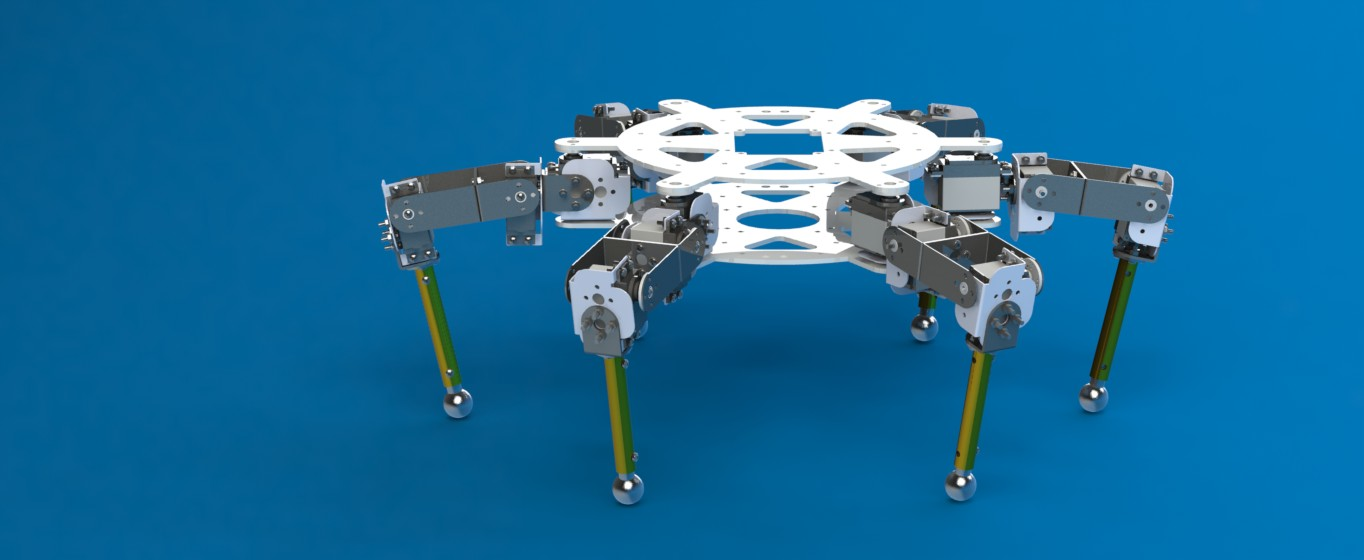
\includegraphics[width=160mm]{Hexapod5}\\}
\caption{CAD модель робота в SolidWorks}
\end{figure}

В данной главе рассмотрен процесс построения динамической модели шестиногого шагающего аппарата с инсектоморфными ногами. Рассмотрены различные кинематические схемы ног аппарата. Приведен аналитический алгоритм синтеза управления движением робота для регулярной походки "трешками" по плоскости. Работоспособность алгоритма подтверждена при помощи компьютерного моделирования в программном комплексе Универсальный Механизм.

При помощи динамической модели были получены такие ключевые параметры, как максимальная грузоподъёмность аппарата при известных параметрах двигателя, максимальная скорость передвижения и соответствующие ей геометрические параметры походки.

За отправную точку создания модели был выбран робот AH3---R фирмы LynxMotion.
Отличительная черта схемы этого робота --- центральная симметрия корпуса. Точки крепления ног образуют правильный шестиугольник. Ноги имеют инсектоморфную кинематическую схему (Рис. \ref{fig:insect}). Вся управляющая электроника, аккумуляторные батареи и средства связи располагаются на верхней и внутренней палубе корпуса аппарата.

\begin{figure}[t]
\center{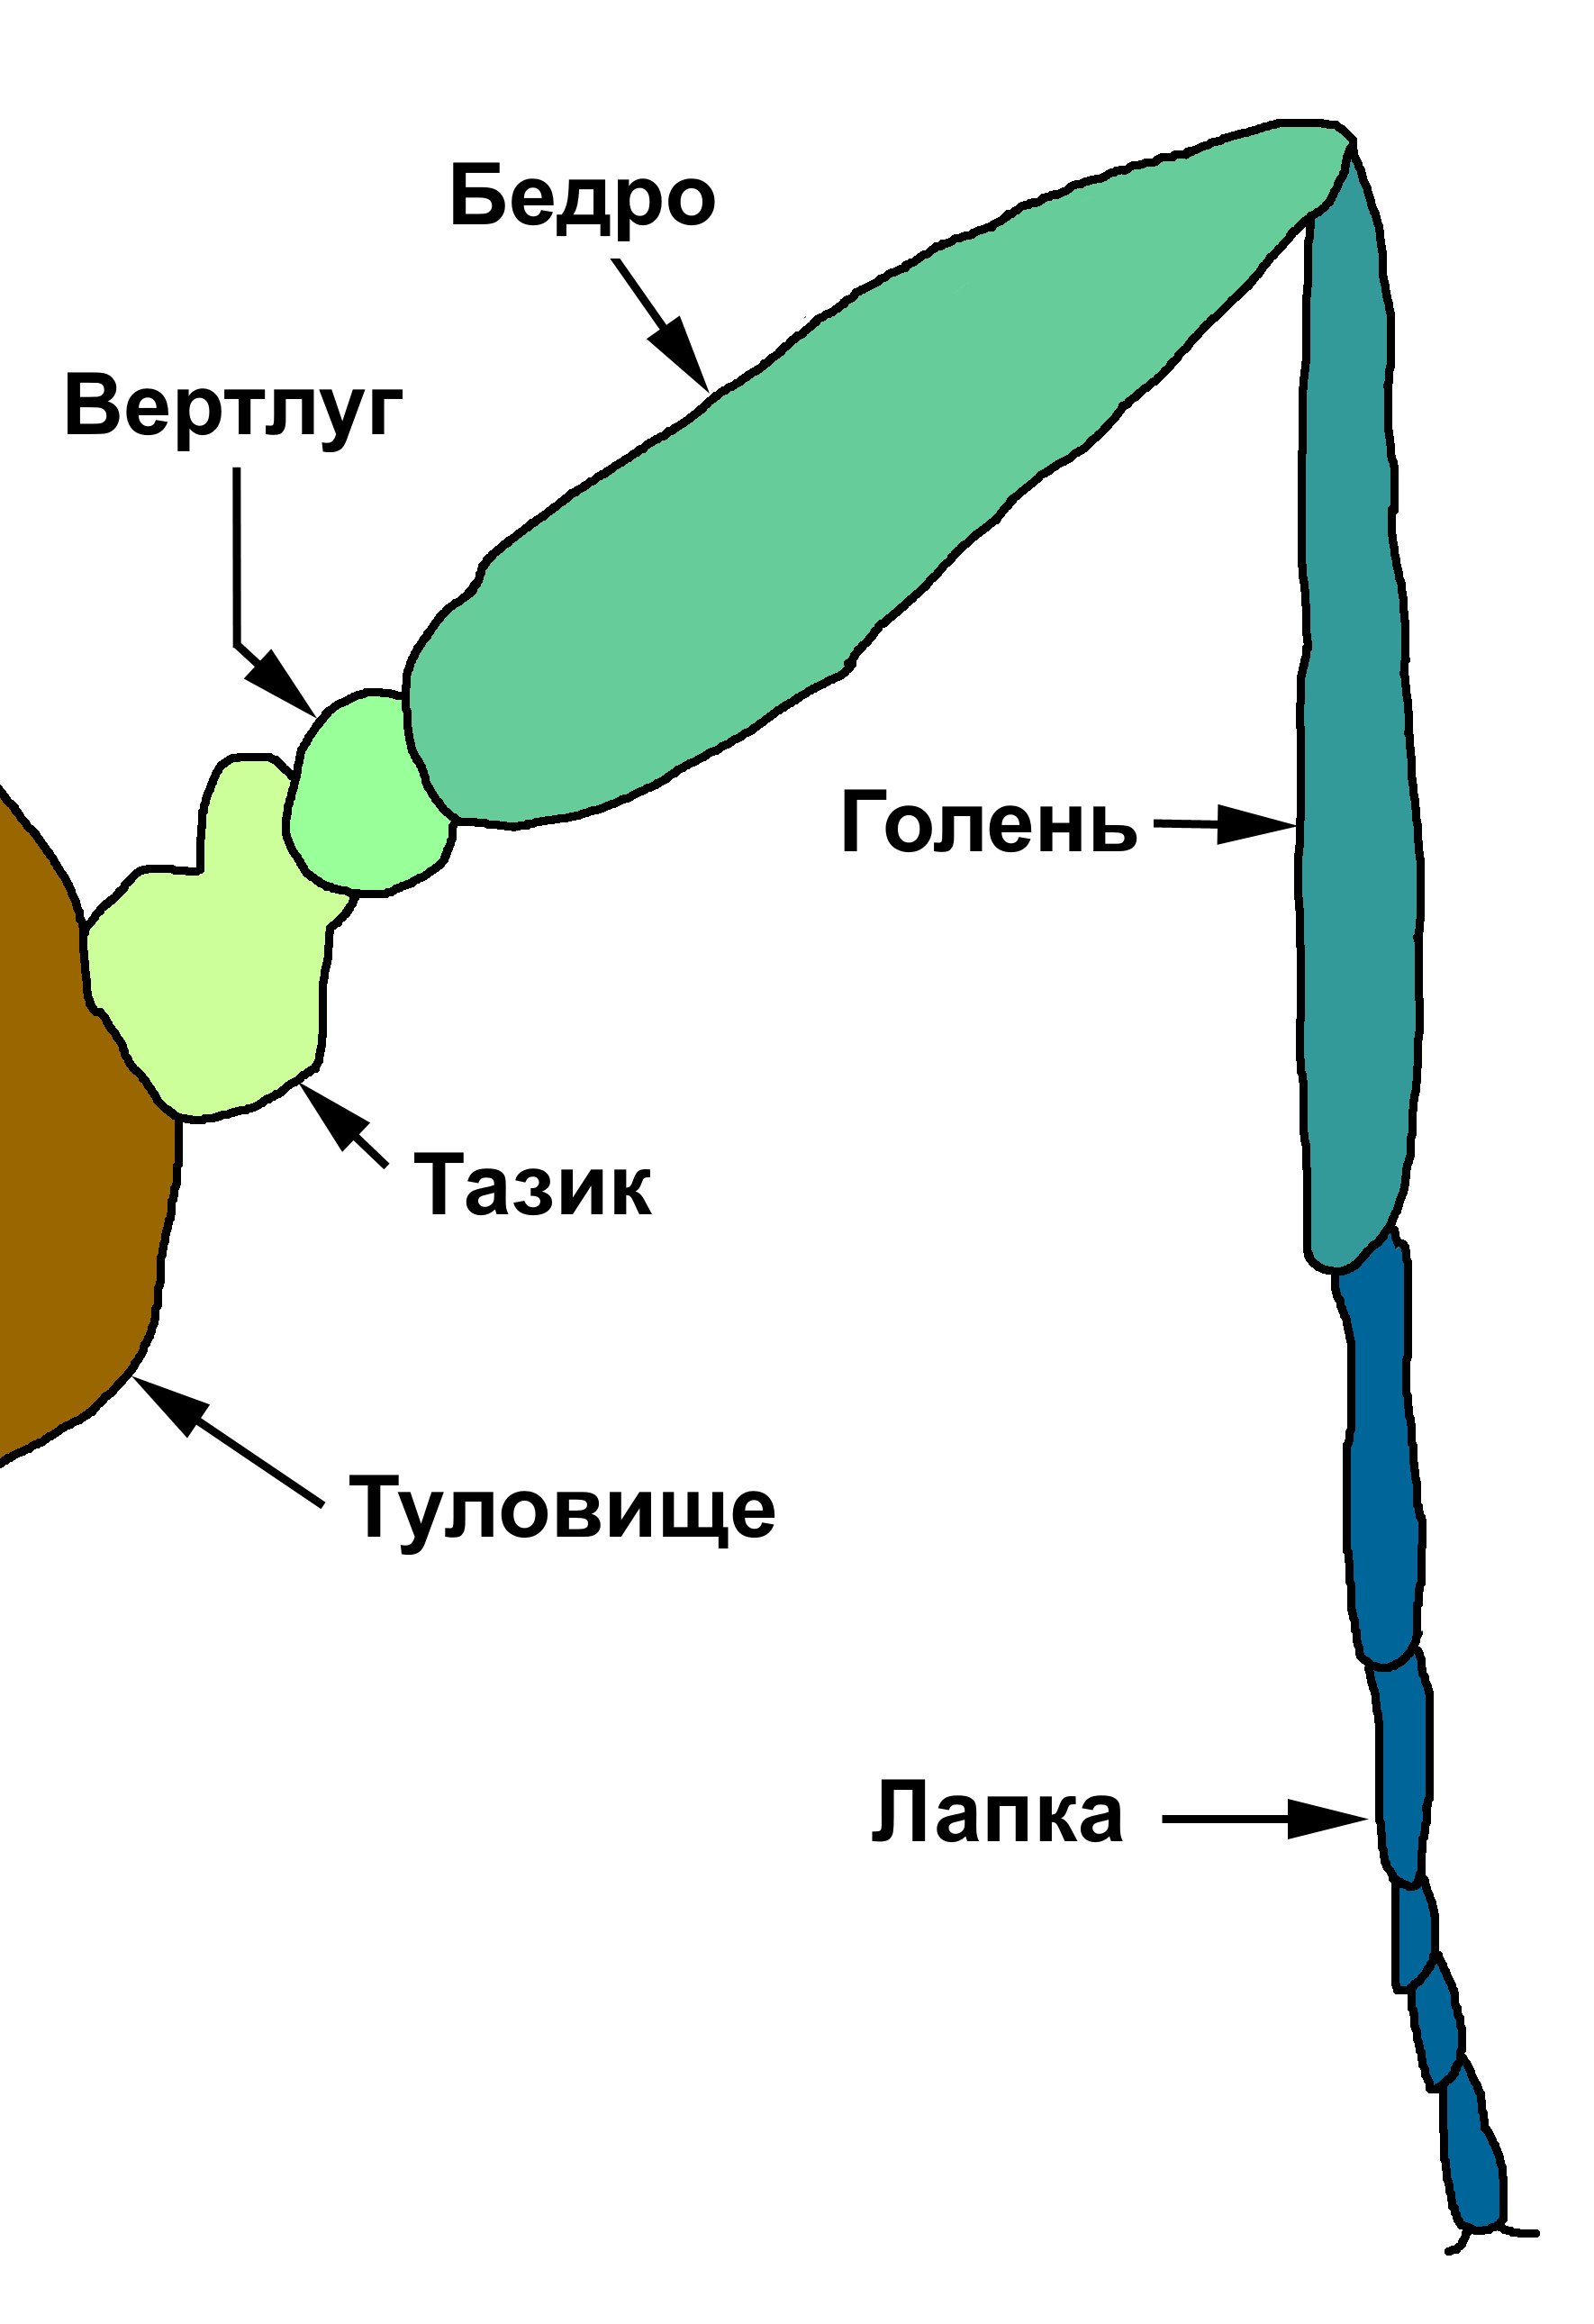
\includegraphics[height=80mm]{InsectLeg}}
\caption{Нога насекомого}
\label{fig:insect}
\end{figure}

\begin{figure}[!h]
\begin{minipage}{0.49\linewidth}
\center{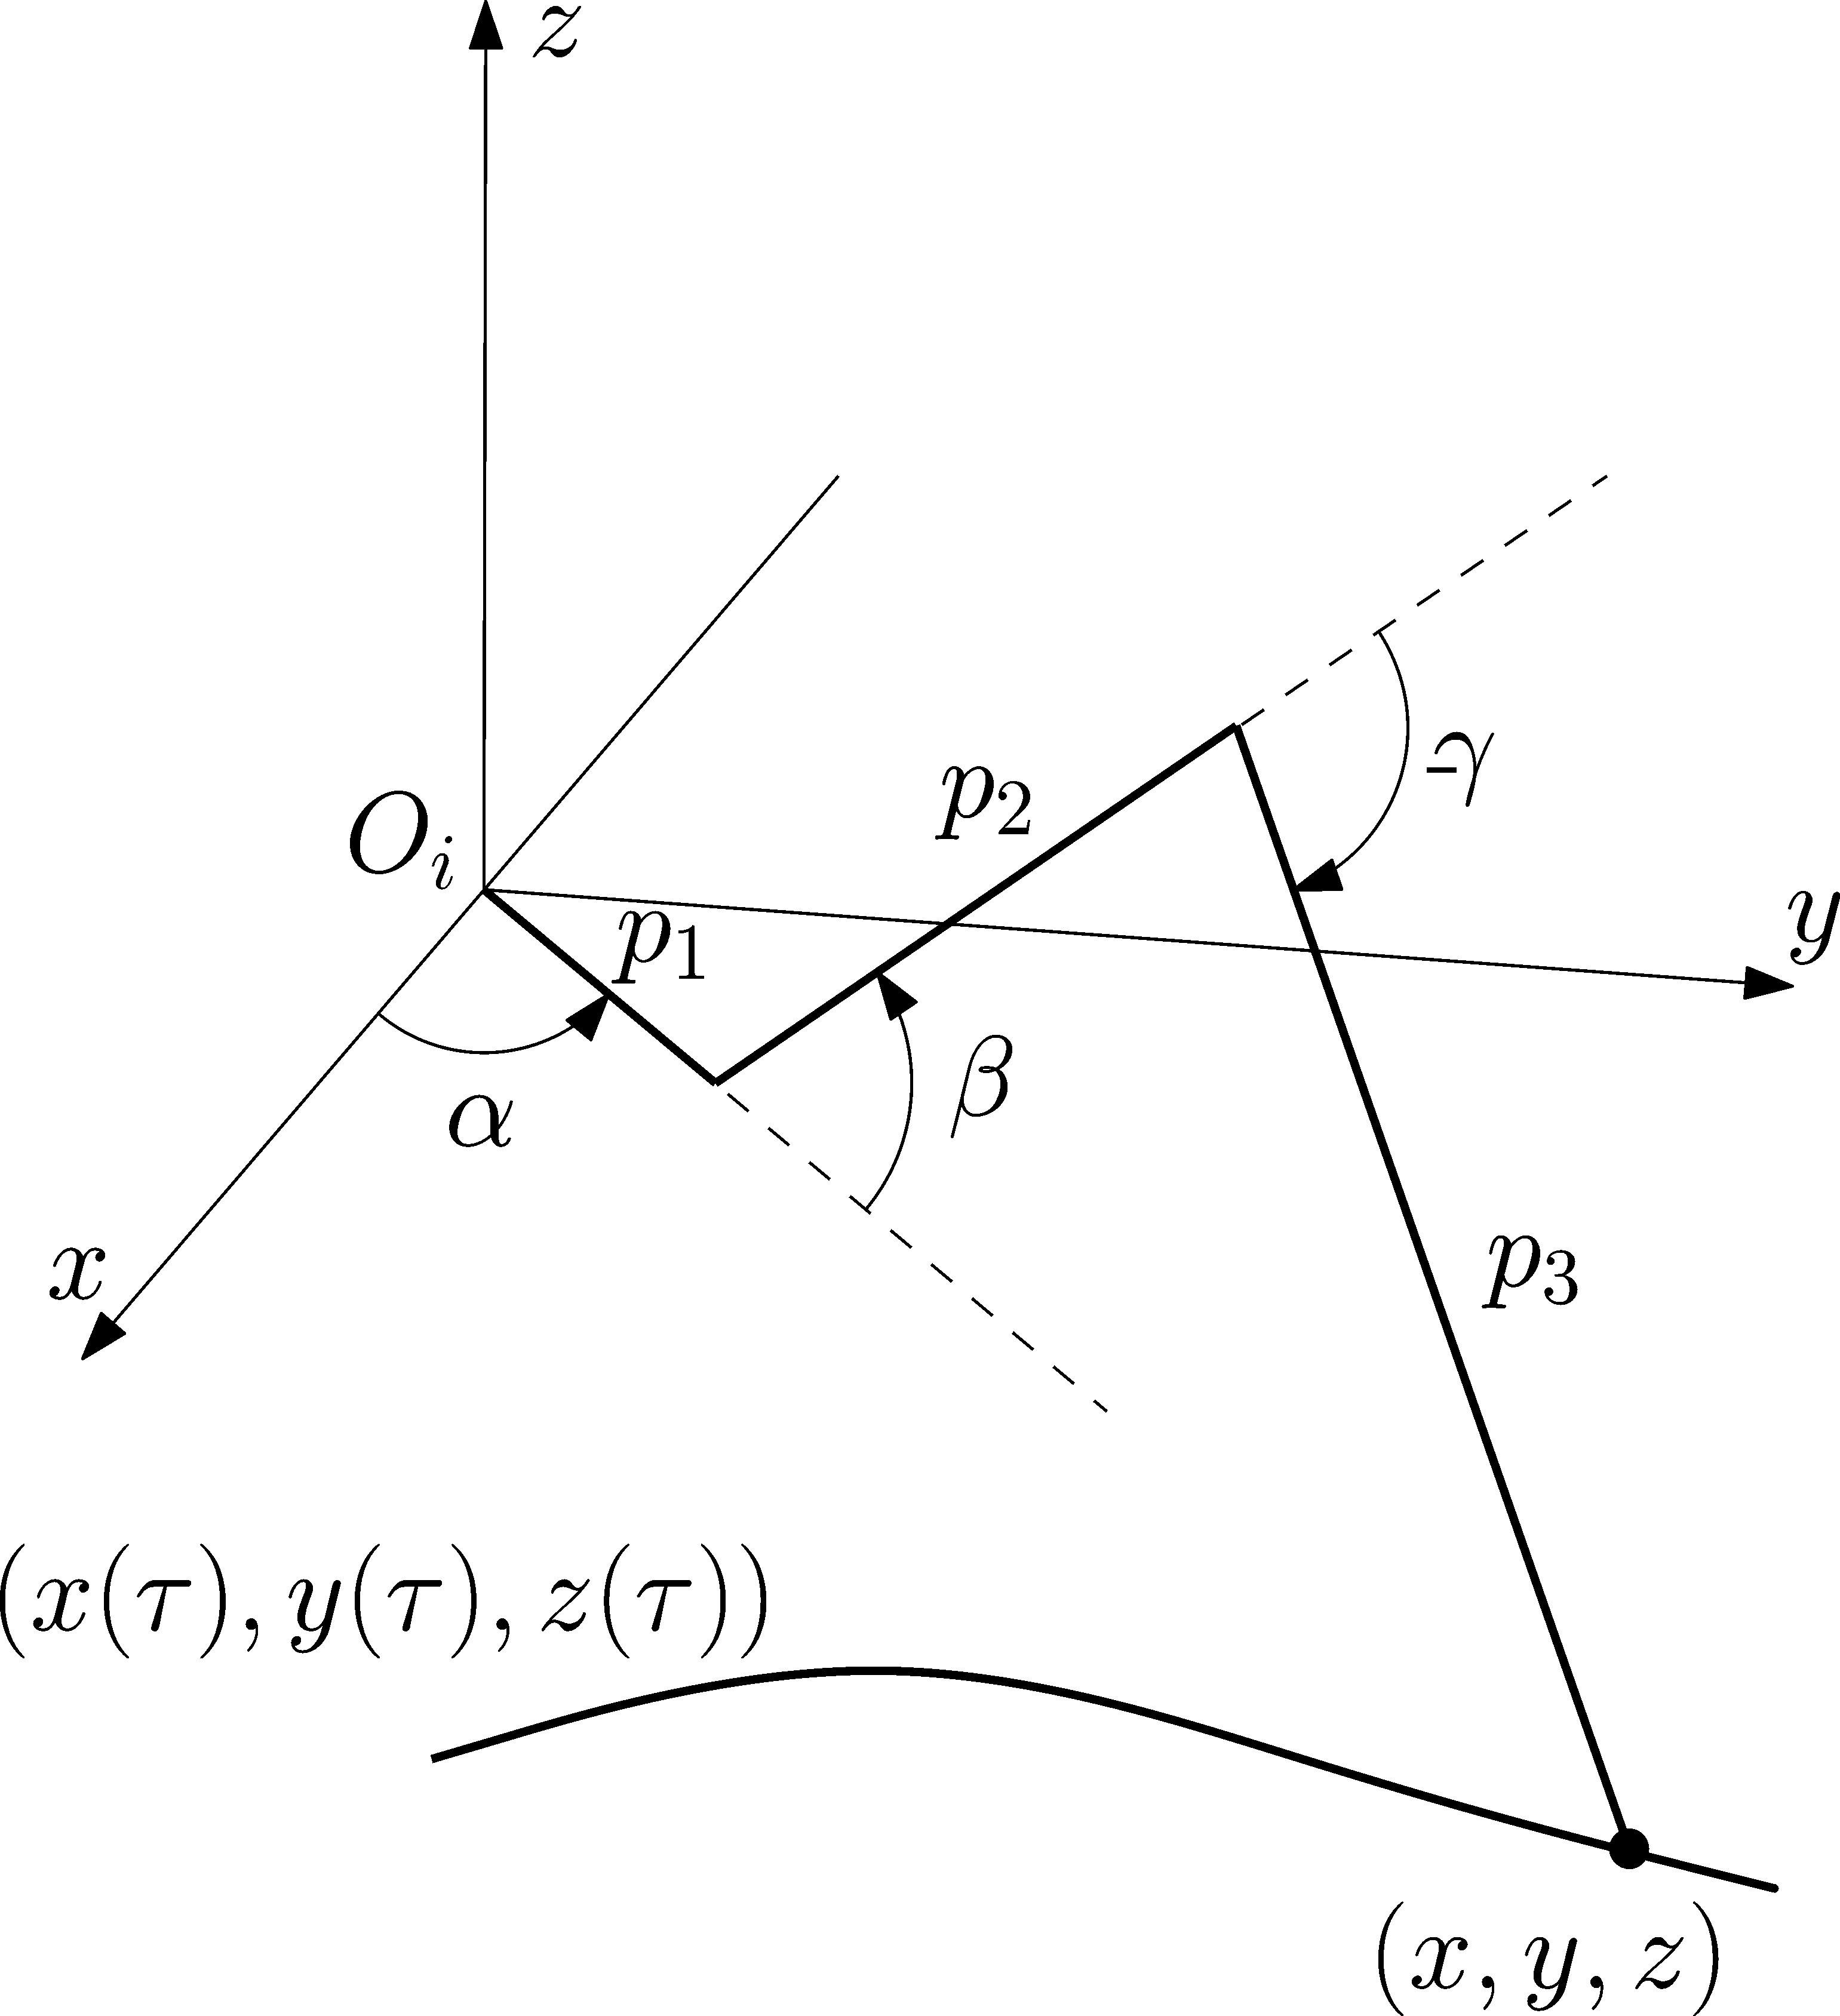
\includegraphics[width=80mm]{Leg}\\}
\end{minipage}
\hfill
\begin{minipage}{0.49\linewidth}
\center{\includegraphics[width=80mm]{CADleg}\\}
\end{minipage}
\caption{Инсектоморфная схема ноги и соответствующая ей CAD модель}
\end{figure}

Конструкция робота имеет модульную структуру. Ноги робота также являются модульными. Каждый модуль собирается из унифицированных деталей, допускающих различные соединения между собой. На сайте разработчиков выложена в открытый доступ обширная библиотека компонентов. Детали изготавливаются из листового материала при помощи лазерной резки на ЧПУ станке, либо печатаются на 3D принтере. Всё вышеперечисленное позволяет легко перестраивать робота и проводить исследование новой кинематики, или синтезировать кинематику робота под определенную задачу. Например, вставлять дополнительные степени свободы, если есть необходимость добавить подвижность в сегмент. Такая модульная конструкция является удобной платформой для отработки алгоритмов управления шагающих аппаратов.


\subsection{Прямая и обратная задача кинематики}

Рассмотрим инсектоморфную схему ноги (\ref{fig:insect}). Нога робота состоит из трех звеньев с длинами $p_1=35$мм, $p_2=75$мм, $p_3=142$мм. Звенья соединены вращательными шарнирами. Звено длины $p_1$ i---ой ноги крепится к корпусу аппарата в точке $O_i$. Ось $Oz$  направлена перпендикулярно горизонтальной плоскости корпуса, ось $Ox$  направлена вдоль радиуса, проведенного из центра корпуса через точку крепления ноги. Аналогичным образом, для каждой ноги задаётся своя система координат (СК). В системах координат, связанных с ногами, удобно задавать шаговый цикл и решать обратную кинематическую задачу.

Напишем прямую задачу кинематики для одной ноги. Требуется определить координаты $(x,y,z)$ конца ноги по углам $(\alpha,\beta,\gamma)$. Звено $p_1$ вращается вокруг оси $O_iz$ в плоскости $O_ixy$. Конец звена $p_1$ имеет координаты:

$$(p_1\,\cos(\alpha),p_1\,\sin(\alpha),0)$$

Звено $p_2$ крепится к подвижному концу звена $p_1$ и вращается относительно точки крепления в вертикальной плоскости, проходящей через звено $p_1$. Свободный конец звена $p_2$ имеет координаты: $$(p_1\,\cos(\alpha)+p_2\,\cos(\beta)\,\cos(\alpha),p_1\,\cos(\alpha)\,\sin(\alpha),p_2\,\sin(\beta))$$

Прямая кинематическая задача для ноги записывается системой уравнений:

\begin{equation}
\left\{
\begin{array}{lcr}
x = \cos(\alpha)(p_1+p_3\,\cos(\beta+\gamma)+p_2\,\cos(\beta))\\
y = \sin(\alpha)(p_1+p_3\,\cos(\beta+\gamma)+p_2\,\cos(\beta))\\
z = p_3\,\sin(\beta+\gamma)+p_2\,\sin(\beta)
\end{array}
\right.
\end{equation}
 
Обратная задача кинематики может иметь до 4 различных решений. Из практических соображений выбирается решение, соответствующее верхнему расположению коленного сустава и естественному повороту сегмента  $p_1$.
В явном виде выбранное решение системы выглядит следующим образом:

\begin{equation}
\left\{
\begin{array}{lcr}
\alpha = \arctan\left(\dfrac{y}{x}\right)\\
\\
\beta = -\arccos\left(\dfrac{x\,\cos(\alpha)+y\,\sin(\alpha)-p_1}{\left((x\,\cos(\alpha)+y\,\sin(\alpha)-p_1)^2+z^2\right)^{\frac{1}{2}}}\right)+\\
\\
+\arccos\left(\dfrac{{p_2}^2+(x\,\cos(\alpha)+y\,\sin(\alpha)-p_1)^2+z^2-{p_3}^2}{2p_2\,((x\,\cos(\alpha)+y\,\sin(\alpha)-p_1)^2+z^2)^{\frac{1}{2}}}\right)\\
\\
\gamma = -\arccos\left(\dfrac{(x\,\cos(\alpha)+y\,\sin(\alpha)-p_1)^2+z^2-{p_2}^2-{p_3}^2}{2p_2p_3}\right)\\
\end{array}
\right.
\label{revkinhexa}
\end{equation}

Заметим, что выражения для углов не зависят от знака координаты $z$. Для решения (\ref{revkinhexa}) предполагалось, что все точки шагового цикла имеют координату $z<=0$. Для случая $z>0$ решение будет отличаться противоположным знаком  при первом слагаемом в выражении для угла $\beta$. Для случая $z>0$ угол $\beta$ будет записываться следующим образом:

\begin{equation}
\begin{array}{lcr}
\beta = \arccos\left(\dfrac{x\,\cos(\alpha)+y\,\sin(\alpha)-p_1}{\left((x\,\cos(\alpha)+y\,\sin(\alpha)-p_1)^2+z^2\right)^{\frac{1}{2}}}\right)+\\
\\
+\arccos\left(\dfrac{{p_2}^2+(x\,\cos(\alpha)+y\,\sin(\alpha)-p_1)^2+z^2-{p_3}^2}{2p_2\,((x\,\cos(\alpha)+y\,\sin(\alpha)-p_1)^2+z^2)^{\frac{1}{2}}}\right)\\
\end{array}
\end{equation}

Для определения области достижимости ноги достаточно рассмотреть плоскость ноги, т.к. вся область достижимости ограничена поверхностью вращения.

\begin{figure}
\center{\includegraphics[width=100mm]{leg_area}}
\caption{Область достижимости инсектоморфной ноги аппарата HexMini}
\label{fig:leg_area}
\end{figure}


На рис. \ref{fig:leg_area} представлено сечение области достижимости для инсектоморфной ноги со звеньями $p_1 = 35$мм, $p_2=75$мм, $p_3=142$мм с учетом геометрических ограничений на шарнирные углы $\alpha, \beta, \gamma$. Геометрические ограничения вычислялись из условия отсутствия пересечения графических образов сегментов в SolidWorks. Ограничения на шарнирные углы вычислены в градусах и взяты с некоторым запасом:

\begin{equation}
\alpha \in [-43^{\circ},43^{\circ}], \beta\in [-45^{\circ},45^{\circ}], \gamma \in [-150^{\circ},150^{\circ}]
\end{equation}

В реальном аппарате необходимо дополнительно предполагать, что на бедренный и коленный шарнир дополнительно накладываются ограничения:
\begin{center}
$|\beta_{max}-\beta_{min}| \leq \dfrac{\pi}{2}-\epsilon$ и $|\gamma_{max}-\gamma_{min}| \leq \dfrac{\pi}{2}-\epsilon$,
\end{center}  
где $\epsilon \approx 10^{\circ}$. Фактическое значение $\epsilon$ зависит от модели сервомашинки.  Из---за физического ограничения на угловую амплитуду сервомашинки рабочая область реальной ноги может отличаться от изображенной на рис. \ref{fig:leg_area}. Далее, в модели не будем учитывать ограничение, возникающее из-за сервомашинок, всегда можно попробовать изменить параметры шагового цикла так, чтобы траектория шагового цикла не выходила из рабочей области ноги.

%\subsection{Обратная кинематика трехзвенной ноги с учётом ошибок}

При проектировании нового аппарата могут произойти ошибки, и произведённый аппарат может отличаться от своей математической модели. Нужно уметь учитывать погрешности при изготовлении аппарата и учитывать ошибки в математической модели, чтобы уметь верифицировать алгоритмы управления.

Рассмотрим случай (рис. \ref{kinerror}) когда контактная точка $K'$ не совпадает с концом третьего звена $K$ кинематической схемы. Пусть со звеном длины $p_3$ связана подвижная система координат $Kx'y'z'$. Пусть точка контакта $K'$ в системе $Kx'y'z'$ имеет координаты ${q_1,q_2,q_3}$. 

\begin{figure}[h]
\center{\includegraphics[width=80mm]{pic4}\\}
\caption{Кинематическая схема ноги со сдвигом контактной точки}
\label{kinerror}
\end{figure}

%Рассмотрим плоскость ноги проходящую через целевую точку на траектории

\begin{figure}[h]
\center{\includegraphics[width=100mm]{pic1}\\}
\caption{Плоскость ноги}
\label{legplane}
\end{figure}

Точка $(\tilde{x},\tilde{z})$ в плоскости ноги (рис. \ref{legplane}) это точка траектории, в которую должна быть приведена контактная точка $K'$, причём контактная точка $K'$ не лежит в плоскости ноги. Решим задачу нахождения углов $\beta$ и $\gamma$. 

Пересчитаем длину звена $p_3$:

\begin{equation}
p_3' = \sqrt{(p_3+q_1)^2+q_3^2}
\end{equation}

Контактная точка ноги $K'$ лежит вне плоскости ноги, поэтому недостаточно совместить проекцию контактной точки $K'\perp$ с $(\tilde{x},\tilde{z})$, нужно сместить конец кинематической схемы к оси вращения угла $\alpha$ так, чтобы расстояние между осью вращения плоскости ноги и контактной точкой стало $r = \sqrt{\tilde{x}^2-q_2^2}$. Обратная задача кинематики решена для плоской ноги с длинами звеньев $(p_1,p_2,p_3')$ для целевой точки $(\sqrt{\tilde{x}^2-q_2^2},\tilde{z})$. Остаётся выполнить коррекцию угла $\alpha$ на угол $-\xi$, где $\sin(\xi) = \dfrac{q_2}{\tilde{x}}$, чтобы совместить контактную точку с целевой.

\begin{figure}[h]
\center{\includegraphics[width=70mm]{pic3}}
\caption{Проекция ноги на горизонтальную плоскость}
\end{figure}

На рисунке проекции ноги на горизонтальную плоскость видно, зачем требуется смещение конца ноги ближе к оси вращения ноги. За счёт этого смещения контактная окружность попадает на окружность радиуса $r = \tilde{x}$ и при повороте перейдёт в точности в целевую точку, лежащую на той же окружности.

Решение задачи в явном виде:

\begin{equation}
\left\{
\begin{array}{lcr}
\tilde{x} = \sqrt{x^2+y^2-q_2^2}\\
\\
p_3' = \sqrt{(p_3+q_1)^2+q_3^2}\\
\\
\tilde{\alpha} = \arctan(\dfrac{y}{x})-\arcsin(\dfrac{q_2}{\sqrt{\tilde{x}^2-q_2^2}})\\
\\
\tilde{\beta} = -\arccos\left(\dfrac{\tilde{x}-p_1}{\sqrt{(\tilde{x}-p_1)^2+z^2}}\right)+\arccos\left(\dfrac{p_2^2+(\tilde{x}-p1)^2+z^2-p_3'^2}{2\,p_2\,\sqrt{(\tilde{x}-p_1)^2+z^2}}\right)\\
\\
\tilde{\gamma} = -\arccos\left(\dfrac{(\tilde{x}-p_1)+z^2-p_2^2-p_3'^2}{2\,p_2\,p_3'}\right)-\arcsin\left(\dfrac{q_3}{p_3'}\right)\\
\\
\end{array}
\right.
\end{equation}

Усложним постановку задачи. Пусть теперь допускаются фиксированные сдвиги в каждом шарнире ноги. Найдем решение обратной кинематической задачи с учетом этих сдвигов. Пусть вектор $(p_{ix},p_{iy},p_{iz})$ отвечает за сдвиг точки крепления $i+1$ сегмента. Компоненты $i$-го вектора сдвига заданы в системе координат связанной с $i$-ым звеном.

%\begin{figure}
%\center{\includegraphics[width = 10cm]{pics/blank_pic.pdf}}
%\caption{Вставить иллюстрацию}
%\end{figure}

Рассмотрим виртуальную плоскость ноги, проходящую через ось вращения угла $\alpha$ перпендикулярно к осям вращения $\beta$ и $\gamma$. Сегменты ноги уже не обязаны лежать в этой плоскости. 

Будем последовательно выполнять преобразования длин сегментов ноги и целевой точки. Сдвинем систему координат ноги так, чтобы ось $Oz$ совпала с осью вращения угла $\alpha$, сегмент $p_1$ неподвижным концом находился в начале системы отсчета. Сдвиг системы координат на вектор $(p_{0x},p_{0y},p_{0z})$ равносилен сдвигу целевой точки ноги на вектор $(-p_{0x},-p_{0y},-p_{0z})$.

\begin{equation}
\left\{
\begin{array}{lcr}
x'_0 = x_0-p_{0x}\\
y'_0 = y_0-p_{0y}\\
z'_0 = z_0-p_{0z}\\
\end{array}
\right.
\end{equation}

Определим новый сегмент $p'_1$. Для этого сдвинем систему координат ноги вдоль оси $Oz$ на величину вертикального сдвига точки крепления шарнира угла $\beta$.

\begin{equation}
z''_0 =z'_0-p_{1z} 
\end{equation}

Новая длина сегмента $p'_1 = p_1+p_{1x}$. Далее, проведем пересчет длин сегментов $p_2$ и $p_3$:

\begin{equation}
\begin{array}{lcr}
p'_2 = \sqrt{(p_2+p_{2x})^2+p_{2z}^2}\\
\\
p'_3 = \sqrt{(p_3+p_{3x})^2+p_{3z}^2}\\
\end{array}
\end{equation}

Контактная точка не лежит в плоскости ноги. Расстояние от контактной точки до плоскости ноги равно $(p_{1y}+p_{2y}+p_{3y})$. Рассмотрим проекцию звеньев ноги на горизонтальную плоскость $Oxy$ в случае, когда проекция контактной точки ноги совпадает с целевой точкой. Точка начала координат, контактная точка и целевая точка образуют прямоугольный треугольник $ABC$. Угол $\angle BAC$ требуется компенсировать чтобы совместить контактную точку ноги с целевой. Угол $\angle BAC = arcsin\left(\dfrac{p_{1y}+p_{2y}+p_{3y}}{\sqrt{{x'}_0^2+{y'}_0^2}}\right)$.

При повороте на угол $\angle BAC$ контактная точка не попадет в целевую точку, нужно скорректировать координаты целевой точки так, чтобы после поворота контактная точка попала в исходную целевую.
В плоскости ноги целевая точка имеет координтаы $(\tilde{x_0}, z_0)$, где $\tilde{x_o} = \sqrt{{x'}_0^2+{y'}_0^2}$. 
Построим окружность в горизонтальной плоскости и с центром в начале координат и радиусом $\tilde{x_0}$. Проведем прямую через точку $B$, параллельно оси $O\tilde{x}$. Ближайшую к вершине $B$ точку пересечения обозначим $D$. Основание $DB$, трапеции $ADBC$, по величине равно корректировке координаты $\tilde{x_0}$. $BD = \tilde{x}_0-\sqrt{\tilde{x}_0^2-(p_{1y}+p_{2y}+p_{3y})^2}$.

\begin{equation}
\tilde{x}' = \sqrt{\tilde{x}_0^2-(p_{1y}+p_{2y}+p_{3y})^2}
\end{equation}

После преобразования целевой точки и длин сегментов, подставим новые значения в выражения для углов $\alpha, \beta$ и $\gamma$.

После вычисления всех углов, выполним корректировку угла $\alpha$, вычтем из него угол $\delta_{\alpha} = \angle BAC$:

$$
\alpha' = \alpha - \delta_{\alpha}
$$

Выполним корректировку угла $\beta$. Из-за сдвига в коленном шарнире, вычисленный угол $\beta$ имеет другую полуось отсчета, повернутую относительно исходной полуоси на угол $\delta_{\beta} = arcsin\left(\dfrac{p_{2z}}{p'_2}\right)$.

$$
\beta' = \beta-\delta_{\beta}\\
$$

Аналогично корректируется угол $\gamma$. При корректировке  угла $\gamma$ нужно учесть сдвиг в коленном суставе и сдвиг контактной точки $\delta_{\gamma} = arcsin\left(\dfrac{p_{3z}}{p'_3}\right)$:

$$
\gamma' = \gamma - \delta_{\beta}-\delta_{\gamma}
$$

\newpage
Решение обратной задачи записывается в виде:
 
\begin{equation}
\left\{
\begin{array}{lcr}
\tilde{x} = \sqrt{(x-p_{0x})^2+(y-p_{0y})^2}\\
\\
\tilde{x}' = \sqrt{\tilde{x}^2-(p_{1y}+p_{2y}+p_{3y})^2}\\
\\
\tilde{z}' = z-p_{0z}-p_{1z}\\
\\
\alpha = arctan\left(\dfrac{y-p_{0y}}{x-p_{0x}}\right)-arcsin\left(\dfrac{p_{1y}+p_{2y}+p_{3y}}{\tilde{x}}\right)\\
\\
\beta = -arccos\left(\dfrac{\tilde{x}'-p_1'}{\sqrt{(\tilde{x}'-p_1')^2+\tilde{z}'^2}}\right)+arccos\left(\dfrac{(\tilde{x}'-p_1')^2+\tilde{z}'^2+{p'}_2^2-{p'}_3^2}{2\,p_2'\sqrt{(\tilde{x}'-{p'}_1)^2+\tilde{z}'^2}}\right)-\\
\\
\hfill -arcsin\left(\dfrac{p_{2z}}{p_2'}\right)\\
\\
\gamma = -arccos\left(\dfrac{(\tilde{x}'-p_1')^2+\tilde{z}'-{p'}_2^2-{p'}_3^2}{2{p'}_2{p'}_3}\right)-arcsin\left(\dfrac{p_{2z}}{{p'}_3}\right)-arcsin\left(\dfrac{p_{3z}}{{p'}_3}\right)\\
\end{array}
\right.
\end{equation}



%\input{arc_leg_kinematics}


\subsection{Шаговый цикл}
\label{sec:step}
При помощи шаговых циклов можно задавать поступательное прямолинейное движение аппарата []. Под поступательные прямолинейным движением понимается движение аппарата вдоль естественных направлений, например, вперед---назад, вправо---влево, при этом корпус аппарата сохраняет ориентацию, а траектории  точек аппарата состоят из прямолинейных участков. Изменение ориентации аппарата осуществляется путём разворота аппарата на месте, во время остановок между прямолинейными участками. Такое "дискретное" управление не соответствует современным представлениям об управления. Исследуем возможность задания произвольного движения аппарата при использовании шаговых циклов.  
%(научная новизна состоит в способе решения задачи произвольного движения) 
Под произвольным движением понимаем одновременное независимое изменение всех 6ти степеней свободы корпуса аппарата: три поступательные координаты центра корпуса и три угла ориентации. Независимое управление сразу всеми шестью степенями свободы корпуса позволит аппарату двигаться по произвольной траектории с произвольным изменением ориентации. В результате, полученное движение аппарата будет более естественным и эффективным в смысле удобства управления, т.к. оператор, при ручном управлении, не будет ограничен в наборе возможных перемещений из текущего положения.

Будем строить алгоритм задания произвольного движения, отталкиваясь от более простых случаев, последовательно наращивая сложность управления и вводя дополнительные параметры шаговых циклов.


{\bf Определение}: Шаговый цикл --- параметрическое семейство замкнутых траекторий в СК, связанной с ногой.
При прохождении ногой одного витка по траектории шагового цикла нога робота совершает один шаг.

\begin{figure}[h] 
\center{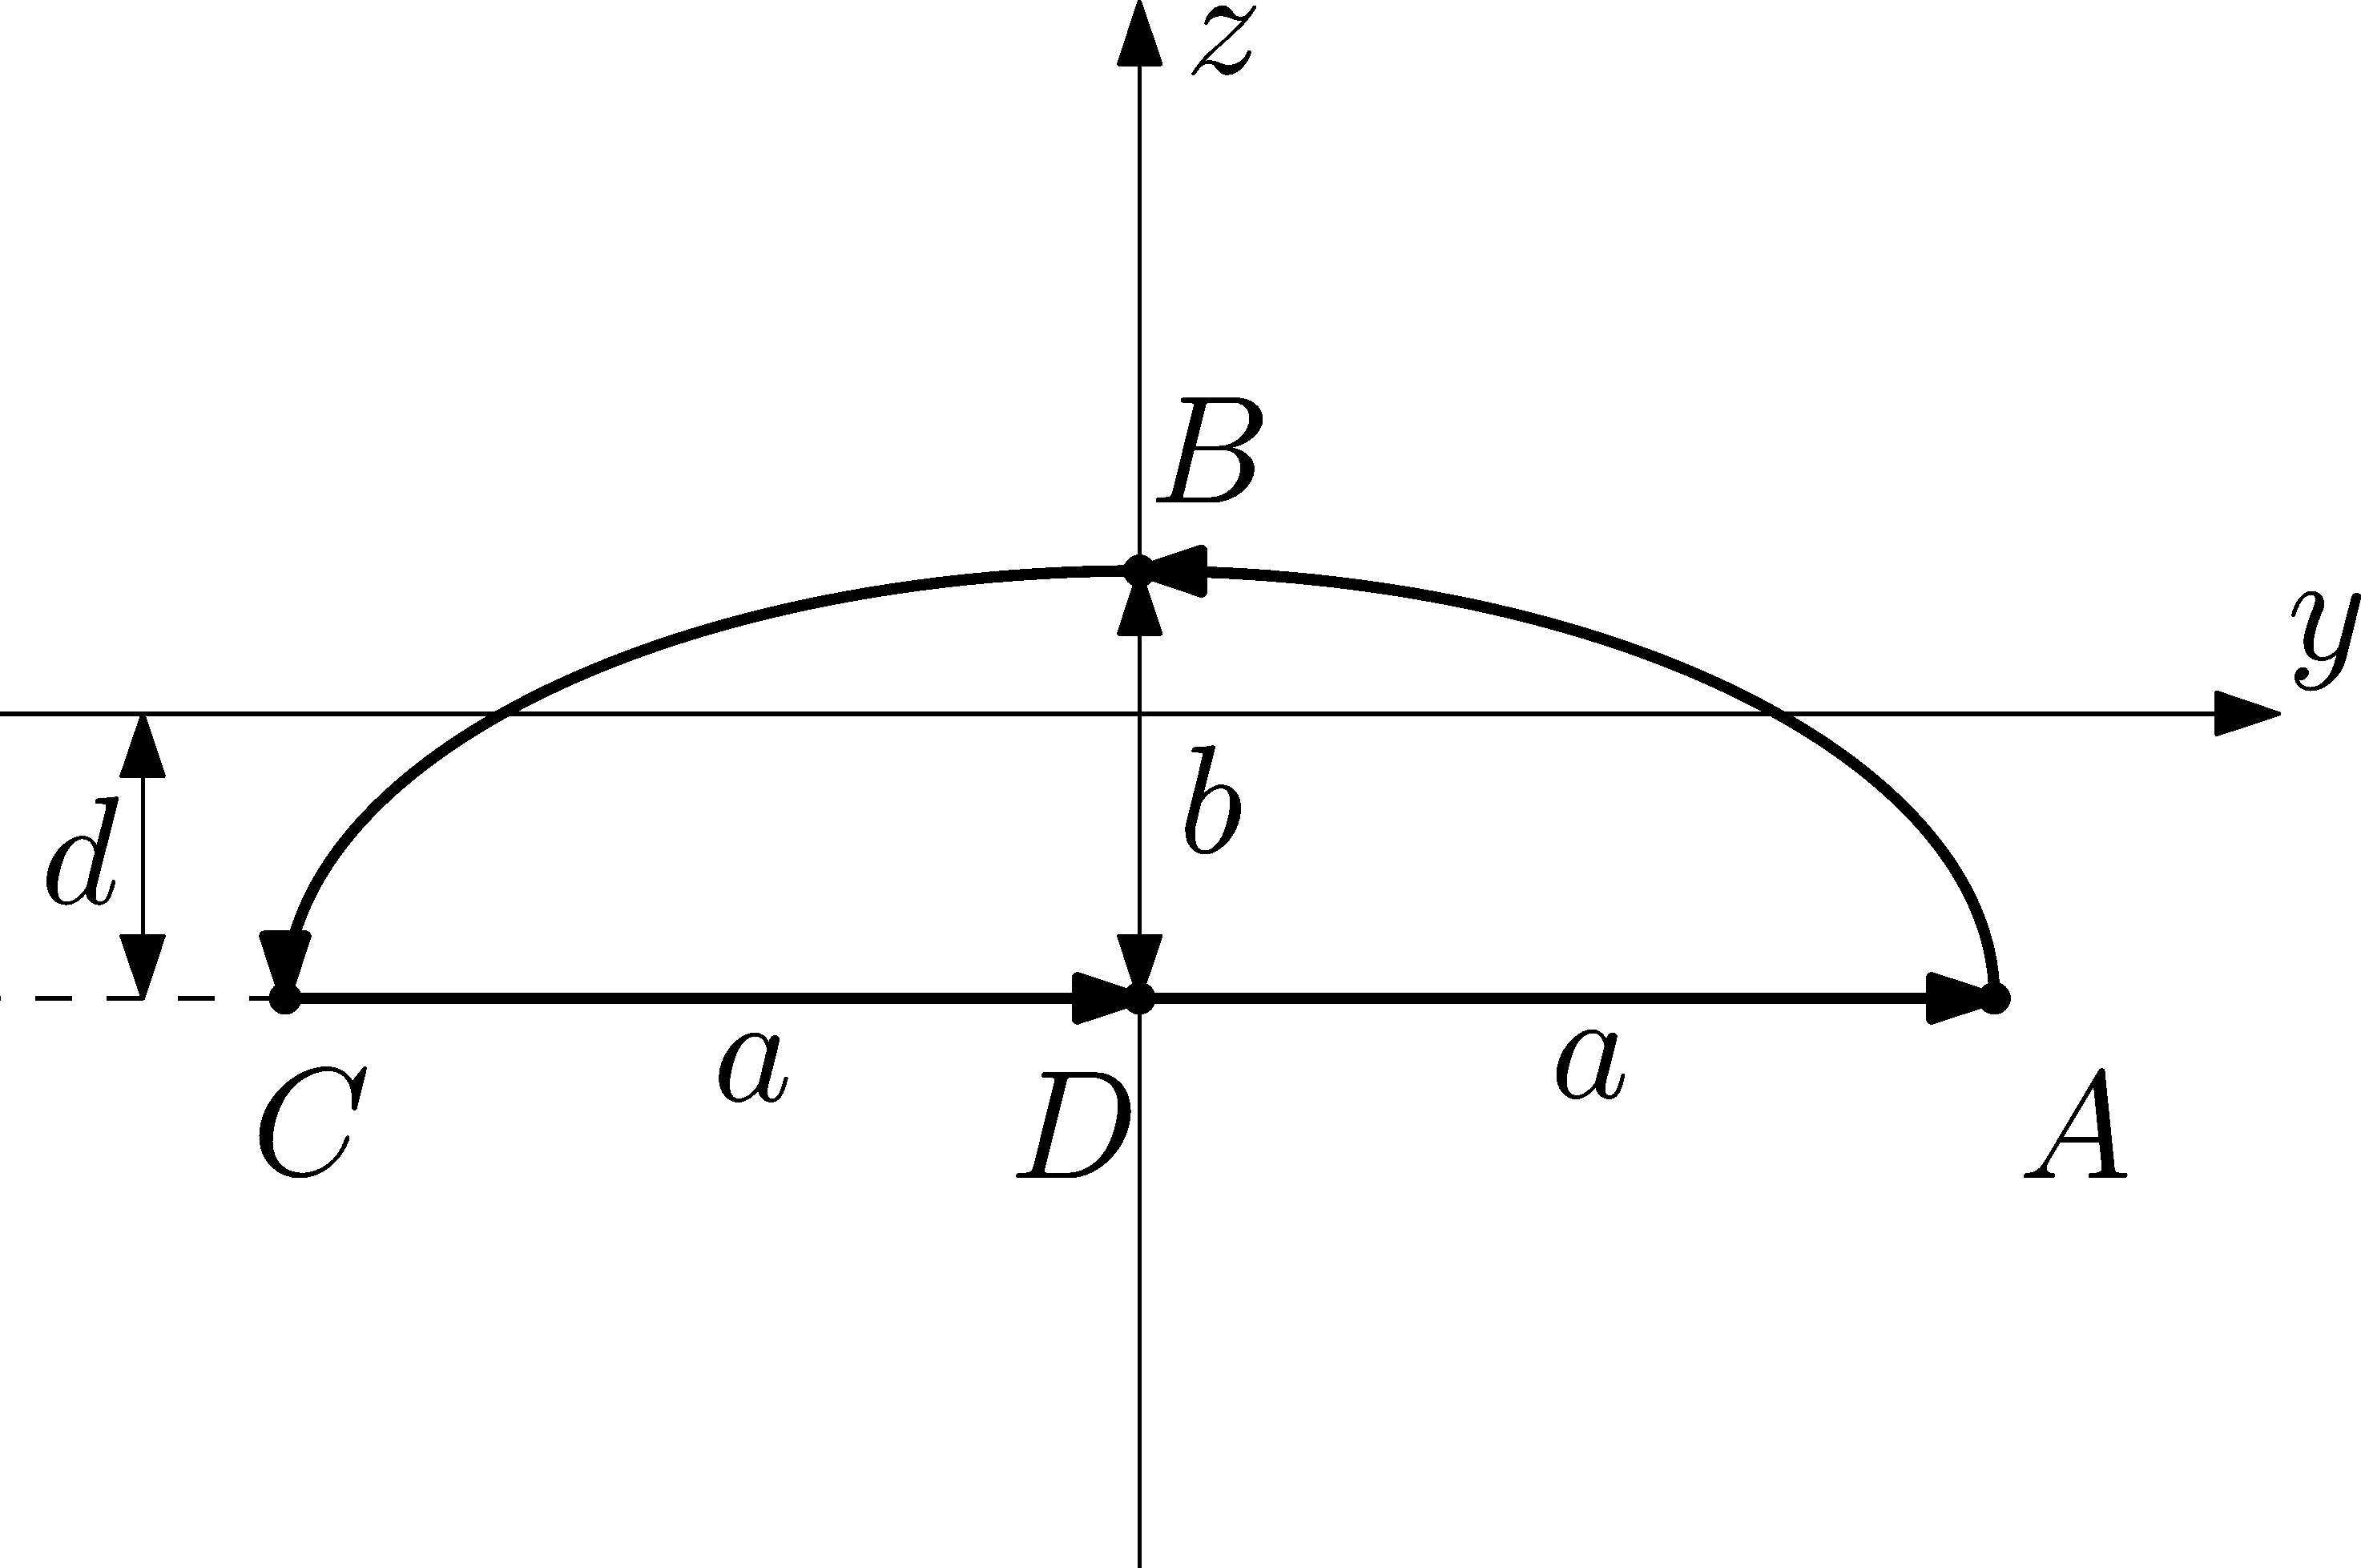
\includegraphics[width = 80mm]{trajectory}\\}
\caption{Шаговый цикл}
\label{fig:step1}
\end{figure}

В качестве шагового цикла (рис. \ref{fig:step1}) выберем половину эллиптической дуги и замыкающую прямую. Часть траектории шагового цикла ноги, соответствующая фазе переноса, лежит в вертикальной плоскости, смещенной на фиксированное расстояние $x_c$  вдоль оси $Ox$ от точки крепления ноги. Стрелками схематически изображено движение по циклу. Замыкающая прямая $CA$ соответствует опорной фазе движения ноги аппарата, эллиптическая дуга $ABC$ соответствует переносной фазе движения ноги, когда нога снимается с опорной поверхности и переносится в новую точку опоры. В зависимости от выполняемого движения корпуса, траектории движения всех опорных ног должны удовлетворять условию не проскальзывания точек контакта.

Основные параметры шагового цикла (рис. \ref{fig:step1}):\\
--- полупериод $W$: время движения стопы в опорной или переносной фазе;\\
--- длина шага $AC = 2a$;\\
--- высота шага $DB = b$;\\
--- вертикальное смещение $d$ центра $D$ шагового цикла относительно точки крепления ноги;\\
--- ширина колеи $x_c$ --- отвечает за замеры опорного многоугольника. \\

Основных параметров не достаточно, чтобы осуществлять произвольное движение аппарата.
Чтобы аппарат совершал перемещения в заданном направлении с заданной скоростью и вращением, шаговые циклы для опорных ног нужно согласовывать, специальным образом подбирая параметры семейств шаговых циклов для разных ног. 

Рассмотрим движение опорных точек в подвижной системе координат, жестко связанной с корпусом робота. Относительно подвижной системы координат контактная поверхность движется как твёрдое тело. Опорные точки перемещаются вместе с опорной плоскостью как одно целое. Для твёрдого тела существует распределение скоростей, подчиняющееся формуле Эйлера (\ref{eq:bodyspeed}).

 \begin{equation}
 \begin{array}{lcr}
 \overline{V_b} = \overline{V_a} + [\overline{\omega} \times \overline{r_{AB}}]
 \end{array}
 \label{eq:bodyspeed}
 \end{equation}
 
Где $A$ и $B$ точки твердого тела, $\omega$ --- угловая скорость тела,$\overline{r}_{AB}$ --- радиус-вектор соединяющий точки $A$ и$B$.
По заданному программному движению корпуса аппарата в каждый момент времени находится распределение скоростей на опорной плоскости относительно подвижной системы координат.

Траектория шагового цикла для фазы переноса записывается в параметрическом виде:

\begin{equation}
\left\{
\begin{array}{lcr}
x = x_c=const,\\
y = a\,\cos(\tau),\\
z = b\,\sin(\tau)-d/\\
\end{array}
\right.,
\label{eq:stand}
 \end{equation}
где $\tau = \dfrac{\pi}{2}\,\left(1-\cos\dfrac{\pi\,t}{W}\right)$, $t$ mod $2\,W\leq W$ и $t$---время, $W$---полупериод одного шага.

Для фазы опоры уравнения шагового цикла имеют вид:

\begin{equation}
\left\{
\begin{array}{lcr}
x = x_c = const\\
y = a\,\cos(\tau)\\
z = -d\\
\end{array}
\right.,
\end{equation}
где $\tau$ берется без изменения из (\ref{eq:stand}), а $t$ mod $2\,W \geq W$.
 
 \begin{figure}[t]
 \center{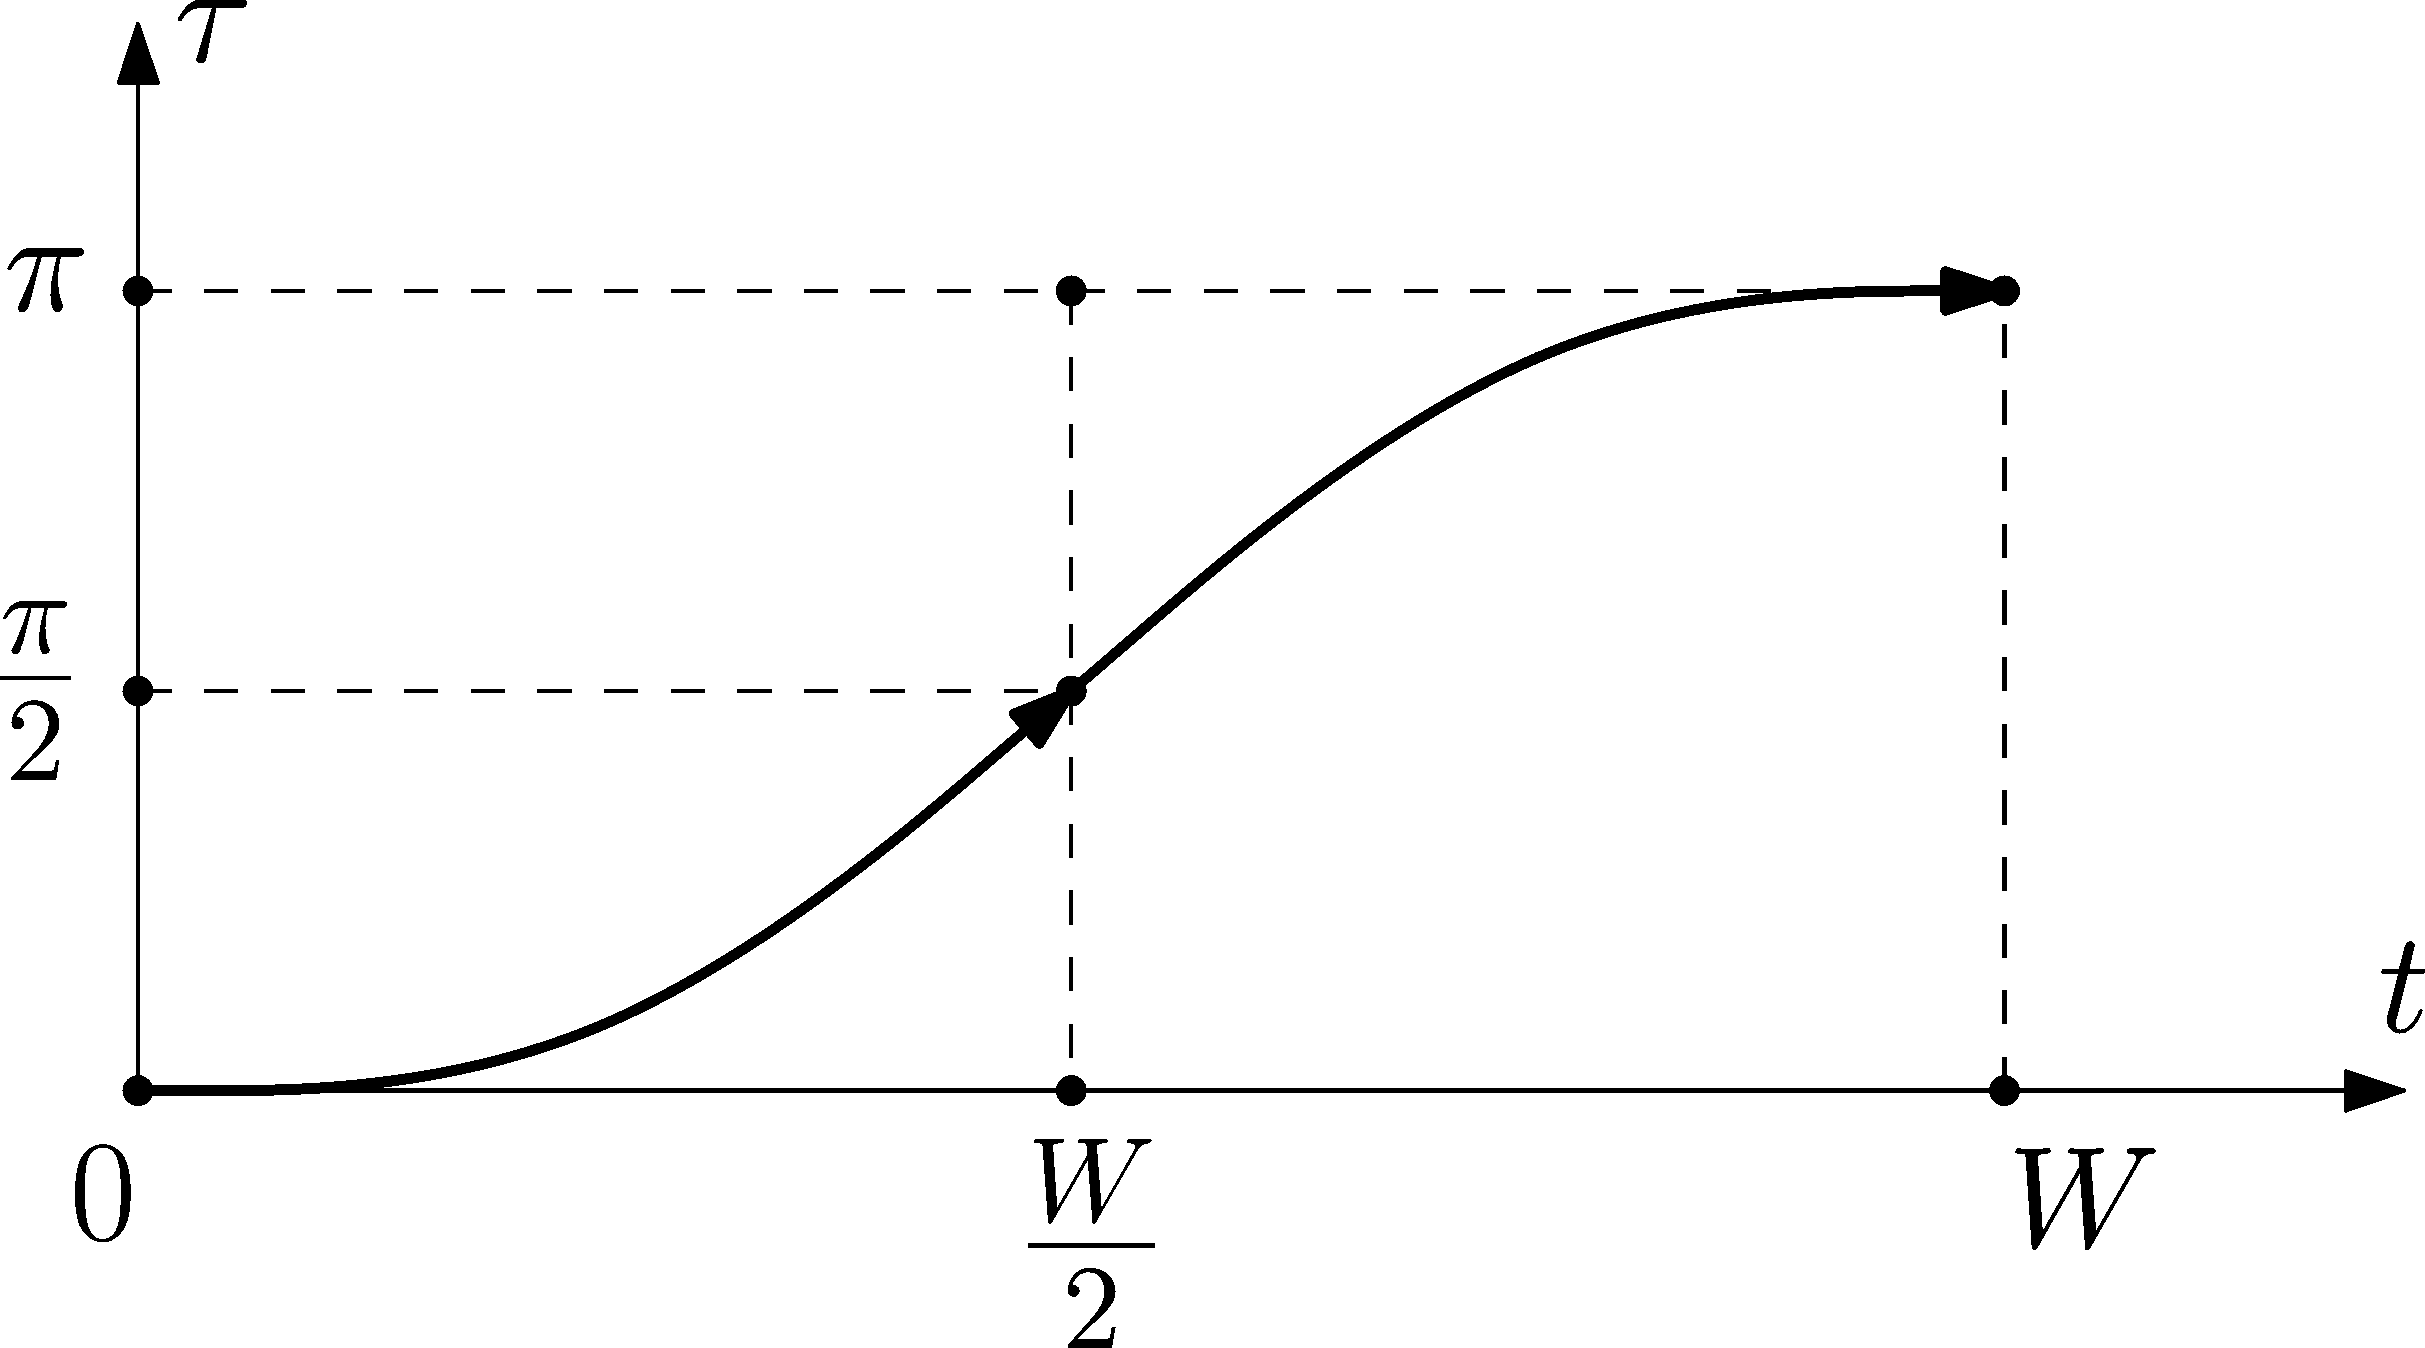
\includegraphics[width = 100mm]{tau}\\}
 \caption{График параметра $\tau$}
 \label{fig:tau}
 \end{figure}
 
График параметра $\tau$ (рис. \ref{fig:tau}) имеет горизонтальные касательные в точках  $t_i = i\,W, i\in\mathbb{Z}$.
Такой выбор параметризации траектории переноса позволяет выполнять постановку и снятие ноги с опорной поверхности с нулевой конечной и начальной скоростью соответственно, таким образом, в системе не происходят удары в моменты постановки и снятия ноги с опорной поверхности. Из---за нулевой скорости стопы в точках снятия и постановки стопы в шаговом цикле возникает остановка всего аппарата, мгновенная скорость аппарата в моменты смены трешек ног равняется нулю. 
%Далее будет показано, как изменить шаговый цикл (рис. \ref{fig:step1}) так, чтобы %избавится от остановок корпуса во время смены трешек.

\subsection{Деформация шаговых циклов}
При поступательном движении, в каждый момент времени поле скоростей опорной поверхности в движении относительно СК, связанной с роботом, представляется однородным полем. В любой паре точек опорной поверхности вектора скорости совпадают по модулю и направлению. Плоскости, в которых расположены траектории движения ног при поступательном перемещении робота, должны быть параллельны векторному полю скоростей контактных точек поверхности в движении относительно робота. Рассчитаем преобразования опорной траектории для $i$---ой ноги при поступательном движении корпуса робота со скоростью $V$ под углом $\xi$  к оси абсцисс.
Угол, на который нужно повернуть плоскость траектории ноги $\theta_i = \xi+\dfrac{\pi}{2}-\eta_i,i = 1\ldots6, \eta_i$---фиксированный угол, отвечающий за поворот СК ноги относительно СК, связанной с корпусом. Вращение шагового цикла нужно выполнить на угол $\theta_i$ вокруг вертикальной оси, проходящей через центр эллипса. Преобразования проводятся в векторном виде при помощи сдвигов на векторы и умножений на матрицы поворотов. После всех преобразований для $i$---ой ноги имеем:

\begin{equation}
\left\{
\begin{array}{lcr}
\hat{x} = x_c-y\,\sin(\theta_i),\\
\hat{y} = y\,\cos(\theta_i),\\
\hat{z} = z.\\
\end{array}
\right.
\end{equation}

Где $y = a_i\,\cos(\tau)$, $a_i$ выбирается из расчёта, что средняя скорость переноса корпуса должна совпадать с заданной скоростью $V$, т.е. за один полупериод $W$ нога проходит расстояние $2a_i=V\,W$. Откуда получаем, что $a_i = \dfrac{V\,W}{2}$.


Усложним модель, пусть теперь во время движения в заданном направлении робот будет вращаться вокруг своего центра с угловой скоростью $\overline{\omega}=(0,0,\omega)$. 

\begin{figure}[h]
\center{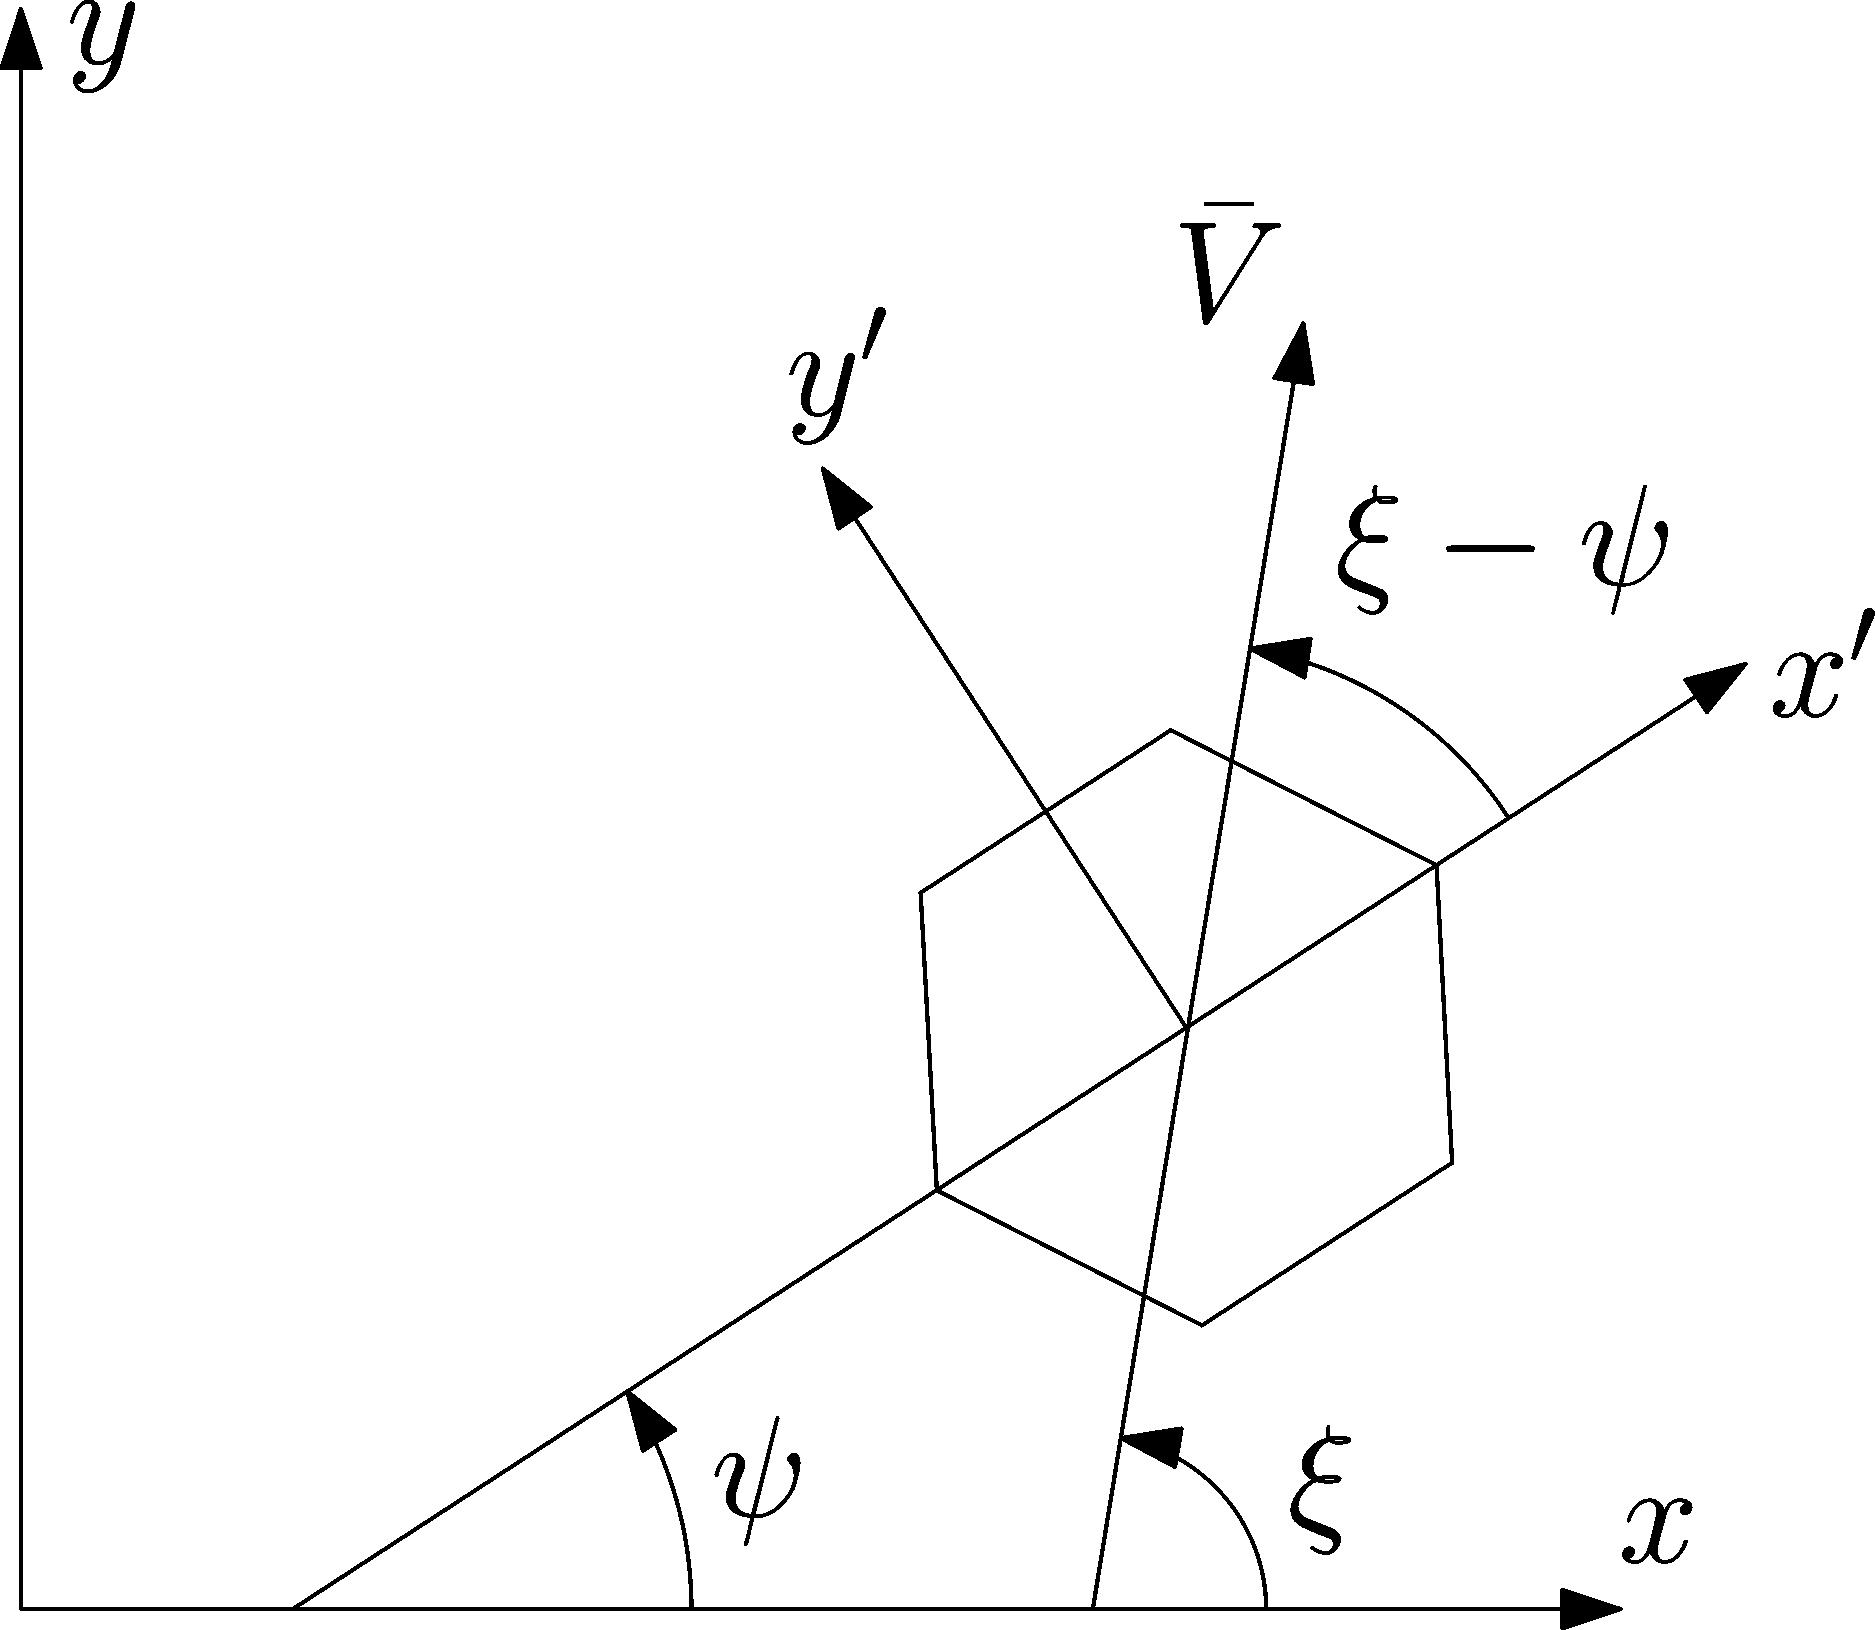
\includegraphics[width = 80mm]{movewithrotation}\\}
\caption{Движение корпуса с вращением}
\end{figure}

При $\omega\neq0$ распределение скоростей на опорной поверхности в относительном движении является центральным. В каждый момент времени, линии тока поля распределения скоростей представляются концентрическими окружностями с одним общим центром --- мгновенным центром скоростей. 
Найдём положение мгновенного центра скоростей в подвижной системе координат в случае $\omega \neq 0$. Координаты положения мгновенного центра скоростей находятся при помощи формулы Эйлера (\ref{eq:bodyspeed}). В системе координат, связанной с корпусом, векторное уравнение запишется в виде системы скалярных уравнений:

\begin{equation}
\left\{
\begin{array}{lcr}
\tilde{x} = -\dfrac{|V|\sin(\xi-\psi)}{\omega}\\
\tilde{y} = \dfrac{|V|\cos(\xi-\psi)}{\omega}\\
\end{array}
\right.
\label{eq:speedcenter}
\end{equation}
 
Система координат корпуса и $i$---ой ноги робота связаны соотношением:
 
 \begin{equation}
 \left(
\begin{array}{c}
x_i\\
y_i\\
z_i\\
\end{array}\right) = \dfrac{d_b}{2}\,
 \left(\begin{array}{c}
\cos(\eta_i)\\ \sin(\eta_i)\\ 0\\
\end{array}\right)
+
\left(
\begin{array}{lcr}
\cos(\eta_i)&-\sin(\eta_i)&0\\ \sin(\eta_i)&\cos(\eta_i)&0\\ 0&0&1\\
\end{array}
\right)\,\left(
\begin{array}{c}
x\\ y\\ z\\
\end{array}
\right)
\label{eq:transform}
\end{equation}
Из (\ref{eq:speedcenter}) и (\ref{eq:transform}) следует, что в системе координат $i$---ой ноги мгновенный центр скоростей будет иметь координаты:
\begin{equation}
\left\{
\begin{array}{lcr}
\tilde{x_i} = \tilde{x}\,\cos(\eta_i)+\tilde{y}\,\sin(\eta_i)-\dfrac{d_b}{2}\\
\tilde{y_i} = -\tilde{x}\,\sin(\eta_i)+\tilde{y}\,\cos(\eta_i)
\end{array}
\right.,
\end{equation}
где $\dfrac{d_b}{2}$ расстояние от центра корпуса аппарата до точки крепления ноги. В силу центральной симметрии корпуса аппарата величина $d_b$ постоянна для каждой ноги.
Траектория $i$---ой ноги в фазе опоры в каждый момент времени --- это окружность (рис. \ref{fig:circ1}) с центром в точке $(\hat{x_i},\hat{y_i})$ и радиусом $R_i=({r_i}^2+{a_i}^2)^\frac{1}{2}$, где $r_i=((\hat{x_i}-x_c)^2+{\hat{y_i}}^2)^\frac{1}{2}$, и $a_i=\dfrac{W|\omega|r_i}{2}, \omega\neq0$.

 \begin{figure}[h]
 \center{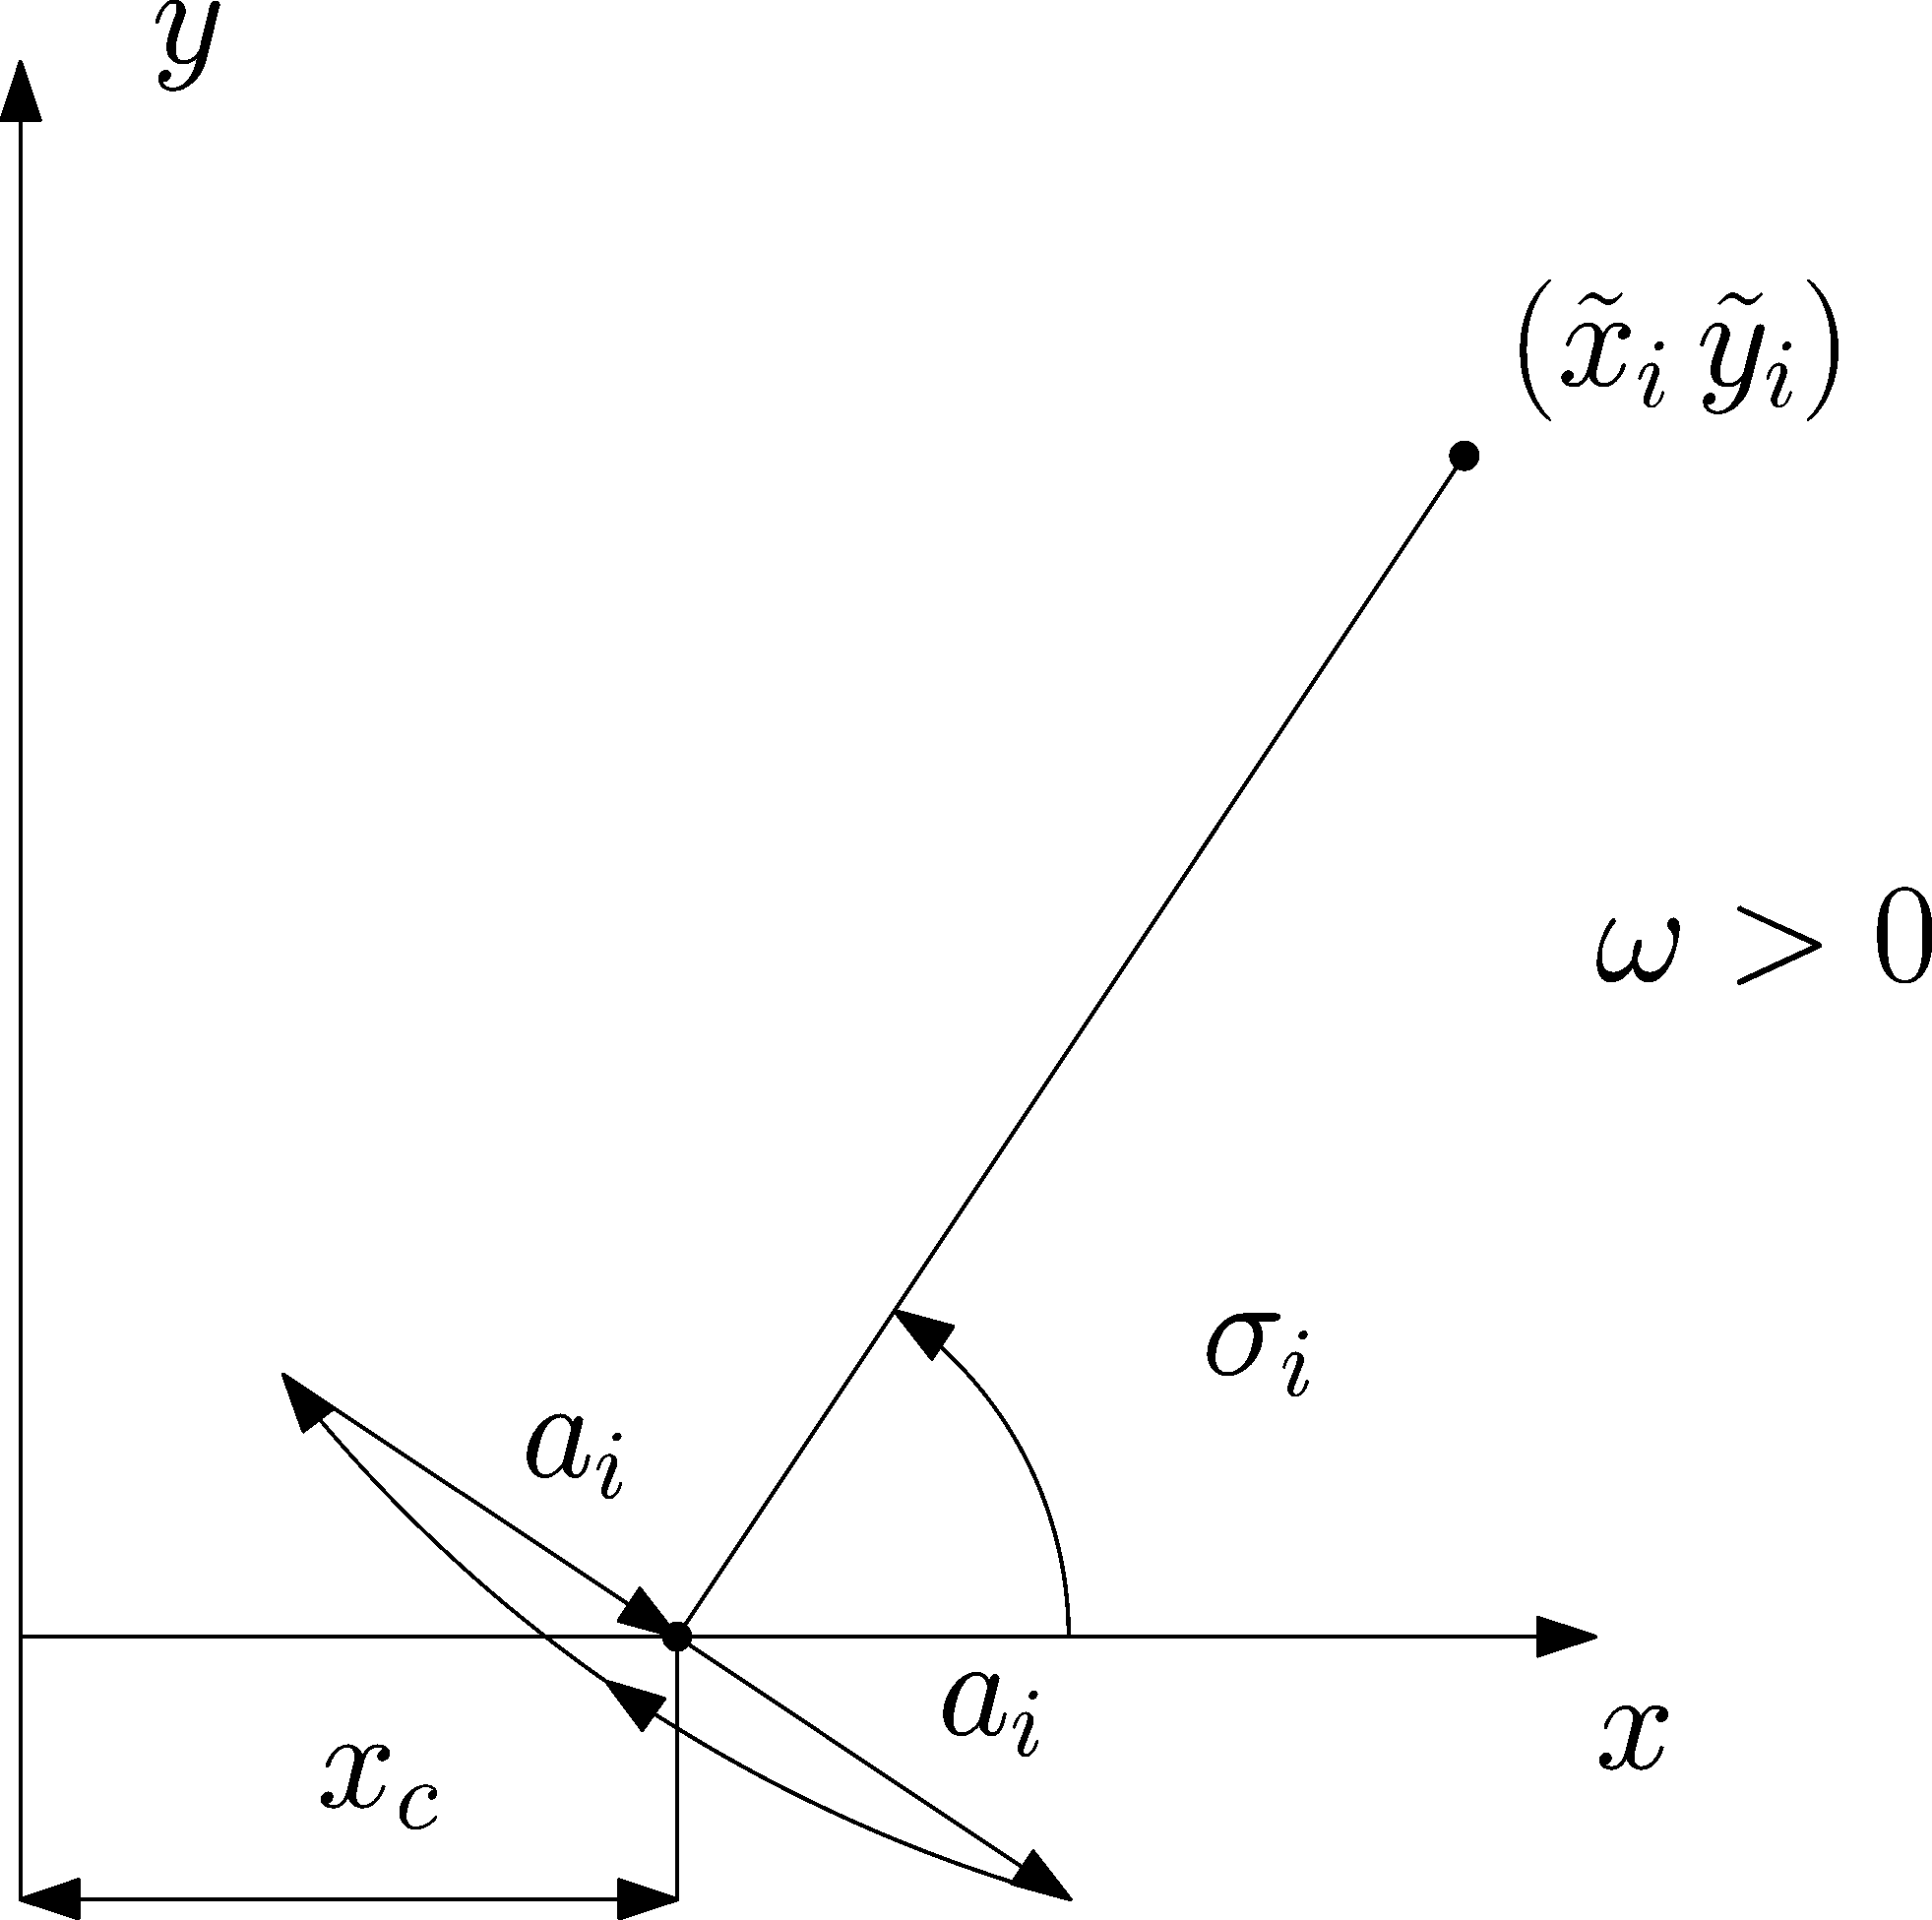
\includegraphics[width=80mm]{sigmaposomega}\\}
 \caption{Опорные траектории при повороте}
 \label{fig:circ1}
 \end{figure}
 
Очевидно, что если параметры движения постоянно изменяются, то будет меняться и поле скоростей на опорной поверхности. Это значит, что в каждый момент времени нужно вычислять положение центра скоростей, определять углы поворота ног $\sigma_i$ и длины шага ног $a_i$.
Параметрические уравнения опорной траектории (рис. \ref{fig:circ1}) записываются в явном виде:

\begin{equation}
\left\{
\begin{array}{lcr}
\hat{x}_i = \cos(\sigma_i)\,sign(\omega)\left(r_i-(R_i^2-y^2)^{\dfrac{1}{2}}\right)-y\,\sin(\sigma_i)+x_c\\
\hat{y}_i = \sin(\sigma_i)\,sign(\omega)\left(r_i-(R_i^2-y^2)^{\dfrac{1}{2}}\right)+y\,\cos(\sigma_i)\\
\end{array}
\right., y = a_i\,\cos(\tau).
\end{equation} 
 
Исследуем поведение опорных траекторий при  $\omega \to 0$.

Найдем предел: 
$$
\lim_{\omega \to 0}a_i = \lim_{\omega\to0}\dfrac{W\omega r_i}{2} = \dfrac{W}{2}\lim_{\omega\to0}\left((\tilde{x_i}-x_c)^2+\tilde{y_i}^2\right)^{\frac{1}{2}}
$$ 

%Для этого подставим выражения для $r_i$ для $\hat{x}$ и $\hat{y}$ .

После всех преобразовании находим, что предел для $a_i$ существует и верно следующее равенство:
$$
\lim_{\omega\to0}a_i = \dfrac{W\,V}{2}
$$

Аналогично находятся пределы:

 $$
 \lim_{\omega\to0}(r_i-\left(R_i^2-y^2\right)^{\frac{1}{2}}) = 0
 $$
 
 $$
 \lim_{\omega\to0}\sigma_i = \theta_i = \xi-\psi+\dfrac{\pi}{2}
 $$
 
 $$
 \lim_{\omega\to0}\hat{x_i} = -y\,\sin(\sigma_i)+x_c
 $$
 
 $$
 \lim_{\omega\to0}\hat{y_i} = y\,\cos(\sigma_i)
 $$
 

 
Откуда следует, что случай поступательного движения является предельным случаем движения робота с вращением корпуса при $\omega\to 0$ .
Доопределим угол поворота опорной траектории следующим образом:

\begin{equation}
\sigma_i = \left\{
\begin{array}{lcr}
\arctan(\dfrac{\tilde{y_i}}{\tilde{x_i}-x_c}),\omega > 0\\
\theta_i = \xi-\psi-\eta_i+\dfrac{\pi}{2},\omega=0\\
\arctan(\dfrac{\tilde{y_i}}{\tilde{x_i}-x_c})+\pi,\omega<0\\
\end{array}
\right.
\end{equation}
 
Теперь $\sigma_i$ буду меняться непрерывно при прохождении точки $\omega=0$. Аналогично, непрерывным образом доопределим длину шага $i$---ой ноги:

\begin{equation}
a_i = \left\{
\begin{array}{lcr}
\dfrac{W|\omega|r_i}{2},\omega\neq0\\
\\
\dfrac{W\,V}{2},\omega=0\\
\end{array}
\right.
\end{equation}
 
При таком определении параметров, шаговый цикл непрерывно зависит от управления  $(\xi,V,\omega)$.
%Причём случай $\omega=0$ является предельным при $\omega\neq0$ при $\omega\to0$.
Можно сказать, что при $\omega=0$ мгновенный центр скоростей находится на бесконечности, а прямые линии тока --- это обобщённые окружности бесконечного радиуса.

На данном этапе синтеза управления проведем моделирование и убедимся в работоспособности приведенного выше принципа построения шаговых циклов для случая поступательного движения корпуса аппарата и для случая сложного движения аппарата, при котором помимо переноса корпуса вдоль заданной траектории происходит вращение корпуса вокруг вертикальной оси с заданной угловой скоростью.

\subsection{Создание динамической модели}
Для создания динамической модели шагающего аппарата используются два программных комплекса. Первый --- САПР SolidWorks. При помощи SolidWorks выполняется проектирование технической документации и проводится предварительное исследование модели. Исследуется геометрия робота, составляется точная 3D модель робота, находятся и оптимизируются габаритные размеры каждого сегмента. Рассчитываются все динамические параметры робота: массы сегментов, моменты инерции, центры масс сегментов. Исследуется кинематика ног: находятся допустимые углы поворота, расположение шарнирных осей в сегментах и взаимное расположение осей вращения.
\begin{table}
\begin{center}
	\begin{tabular}{|c|c|}
	\hline
	  Масса аппарата & 2831гр\\
	  \hline
	  Масса корпуса & 750гр\\
	  \hline
	  Масса одной ноги & 418гр \\	  
	  \hline
	  Масса снаряжения & $\approx$ 500гр\\
	  \hline
	  \end{tabular}
	  \label{tab:masses}
\end{center}
\caption{Массы звеньев аппарата}
\end{table}

\begin{table}	  	  
\begin{center}
\begin{tabular}{|c|c|}
	\hline
	Масса корпуса & 750гр\\
	\hline
	 \multirow{3}{*}{Главные моменты инерции корпуса} & $I_x$=4181316 гр$\cdot$см$^2$\\ 
	 &$I_y$=4199356 гр$\cdot$см$^2$\\ 
	 & $I_z$=7823359 гр$\cdot$см$^2$\\
	  \hline
	  \multirow{3}{*}{Главные моменты инерции таза}  & $I_x$=10952.75гр$\cdot$см$^2$\\
	  & $I_y$=27082.01 гр$\cdot$см$^2$\\
	  & $I_z$=29682.07 гр$\cdot$см$^2$\\
	  \hline
	 \multirow{3}{*}{Главные моменты инерции бедра} & $I_x$=4181316 гр$\cdot$см$^2$\\ 
	 & $I_y$=4199356 гр$\cdot$см$^2$\\
	 & $I_z$=7823359гр$\cdot$см$^2$\\
	  \hline
	 \multirow{3}{*}{Главные моменты инерции голени} & $I_x$=4181316 гр$\cdot$см$^2$\\
	 & $I_y$=4199356 гр$\cdot$см$^2$\\
	 & $I_z$=7823359 гр$\cdot$см$^2$\\
	  \hline	  
	\end{tabular}
	\label{tab:dinam_par_table}
\end{center}
\caption{Таблица расчётных динамических параметров }
\end{table}

Вычисление динамических параметров происходит при помощи встроенных в SolidWorks функций анализа. Задавая геометрический образ каждой детали и материал, из которого сделана деталь, можно вычислить массу детали, положение центра масс, найти главные моменты инерции и главные оси. Все вычисления выполняются автоматически для каждой детали, нужно только указать, к какой системе координат выполнить привязку измеряемых величин, т.е. относительно какого репера будут вычисляться координаты центра масс, компоненты тензора инерции, главные оси. Для сложных сборок узлов аппарата выполняются аналогичные операции.

\begin{table}
\begin{center}
	\begin{tabular}{|c|c|c|c|}
	\hline
	\multicolumn{2}{|c|}{Масса аппарата} & Корпус $\times$ 1 &  Ноги $\times$ 6\\  \hline
	\multicolumn{2}{|c|}{3.258кг}               & 0.750кг                 & 2.508кг              \\	\hline
	\multicolumn{2}{|c|}{100\%}                 & 23\%                     & 77\%                  \\	\hline \hline
	Нога     & Таз             & Бедро                    & Голень              \\ \hline
	0.418кг & 0.2кг & 0.138кг & 0.08кг\\	\hline
	100\%&47\%&33\%&20\%\\	\hline
	\end{tabular}
	\label{tab:masses_ratio}
\end{center}
\caption{Соотношение масс сегментов}
\end{table}

Расчётная масса снаряженного аппарата 3,25 кг, диаметр шестиугольника, образованного точками крепления ног аппарата, составляет 273мм. Вес одной ноги составляет 418 грамм. Масса корпуса 750гр. Длины сегментов ноги $p_1=35$мм, $p_2=75$мм, $p_3=142$мм. Из таблицы (таб. \ref{tab:masses_ratio}) видно, что на массу всех ног приходится доля в 77\% от всей массы аппарата. Самый тяжелый сустав в ноге --- тазобедренный, на него приходится 50\% массы ноги. Распределение массы существенно при работе различных алгоритмов стабилизации. Например, требуется стабилизировать положение аппарата за счёт подвижек корпуса. Если оказалось, что масса корпуса не существенна по сравнению с массой ног, то следует пересматривать компановку робота, проводить перераспределение массы робота и стараться переместить тяжёлые детали на корпус аппарата --- сделать корпус более массивным или, наоборот,  стараться облегчить ноги, путём изменения конструкции, использованием более лёгких материалов.


После всех подготовительных работ выполняется экспорт модели в программный пакет Универсальный Механизм.

\begin{table}
\begin{center}
	\begin{tabular}{|c|c|c|c|}
	\hline
	\multirow{2}{*}{Аппарат} & Время CPU &Число операций  & Время CPU одного \\ &вывода уравнений &с плавающей запятой &шага интегрирования\\
	\hline
	HexaMini&2,046 с&8673шт&0.0023088с\\ 
	\hline
	\end{tabular}
\end{center}
\caption{Протокол синтеза и компиляции уравнений движения}
\end{table}

Для простоты предполагается, что взаимодействие ноги осуществляется по простейшей стандартной модели Универсального Механизма: Точка---Плоскость. В модели Точка---Плоскость нога взаимодействует с опорной поверхностью в одной изолированной точке. Нормальная составляющая силы реакции опоры вычисляется в соответствии с вязко---упругой моделью, касательная составляющая реакции в соответствии с моделью сухого трения:

$$
N = -c\,\delta_z-d\,\dot{\delta}_z, {F_f} = \left\{
\begin{array}{lcr}
-fNv/|v|, |v|>v_f\\
-fNv/v_f,|v|\leq v_f\\
\end{array}
\right.
$$




\begin{figure}
\center{\includegraphics[width = 80mm]{contact}}
\caption{Схема контактного взаимодействия Точка---Плоскость}
\end{figure}
 
 
\begin{figure}[h]
\center{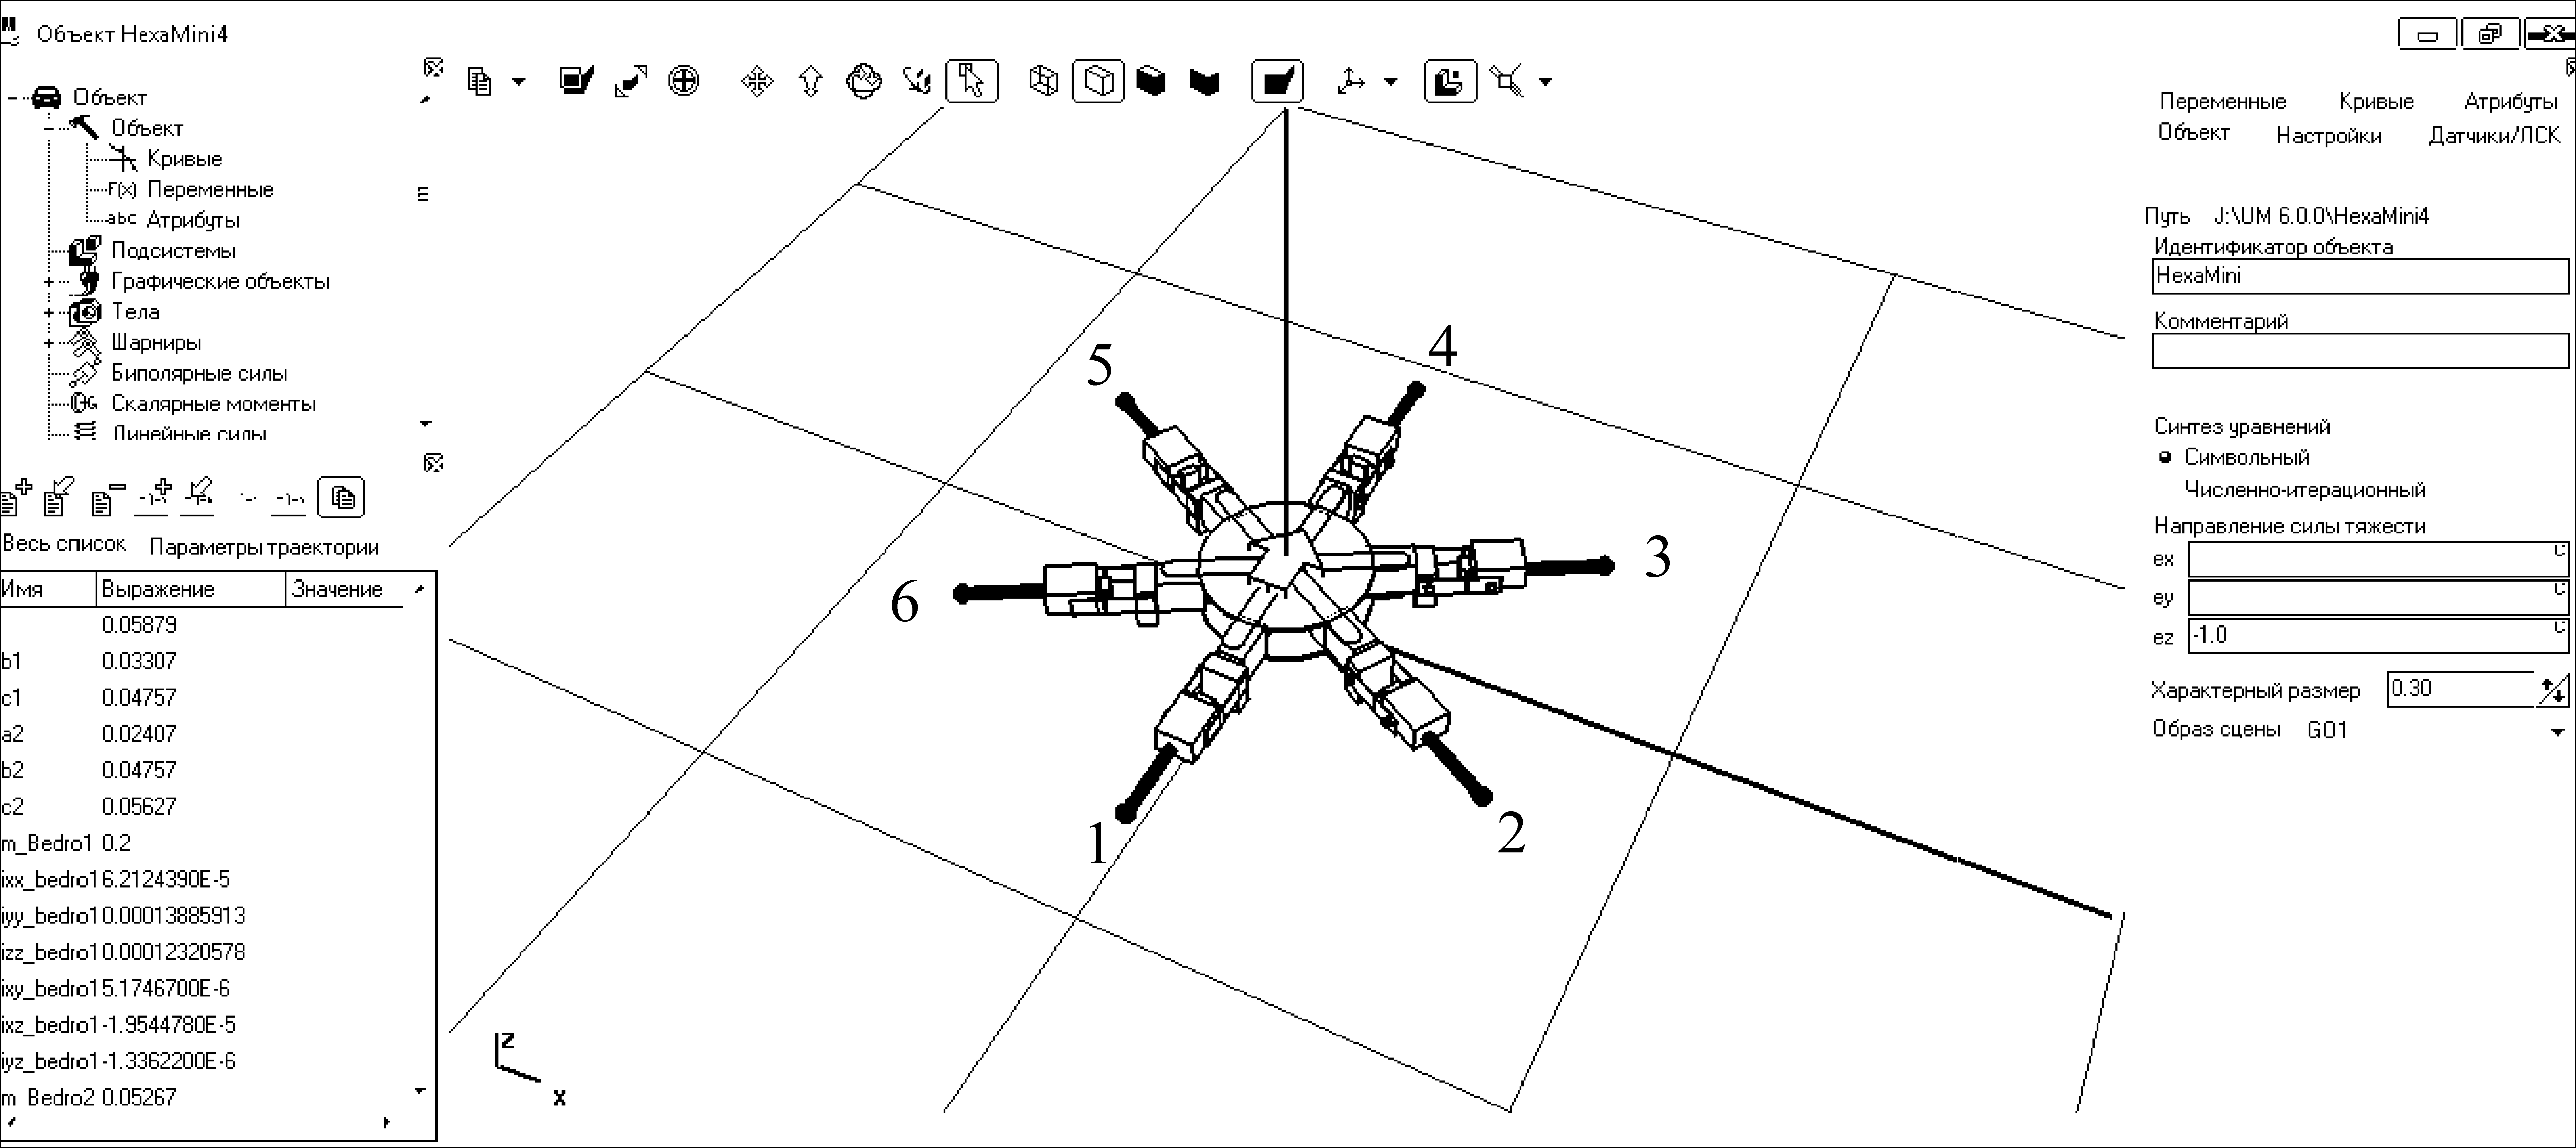
\includegraphics[width=160mm]{UM2}}
\caption{Модель аппарата в ПК УМ}
\label{fig:UM}
\end{figure}  

Для шестиногого аппарата существует множество вариантов возможных походок. Рассмотрим, так называемую, походку "трешками". Ноги разбиваются на две группы, с чётными и нечетными номерами ног (рис. \ref{fig:UM}). В то время как группа ног с нечётными номерами находится в фазе опоры, группа с чётными номерами выполняет фазу переноса. После завершения фаз группы меняются ролями и т.д.


\newpage
\subsection{Моделирование}

Рассмотрим результаты моделирования модели аппарата HexMini с шаговым циклом из пункта \ref{sec:step} Модельные эксперименты --- движение робота по окружности. Проведем эксперименты для двух случаев: для поступательного движение корпуса и для движения корпуса по траектории с одновременным вращением вокруг вертикальной оси.


\label{sec:exper1}
Поступательное движение по окружности (рис. \ref{fig:exper1}) задаётся изменением курсового угла движения с постоянной скоростью и нулевой угловой скоростью корпуса:

\begin{center}
$\xi = \dfrac{2\pi}{30}\,t, V = 0.04$м/с$, \omega = 0, t = 30$с
\end{center}

 \begin{figure}[h]
\center{\fbox{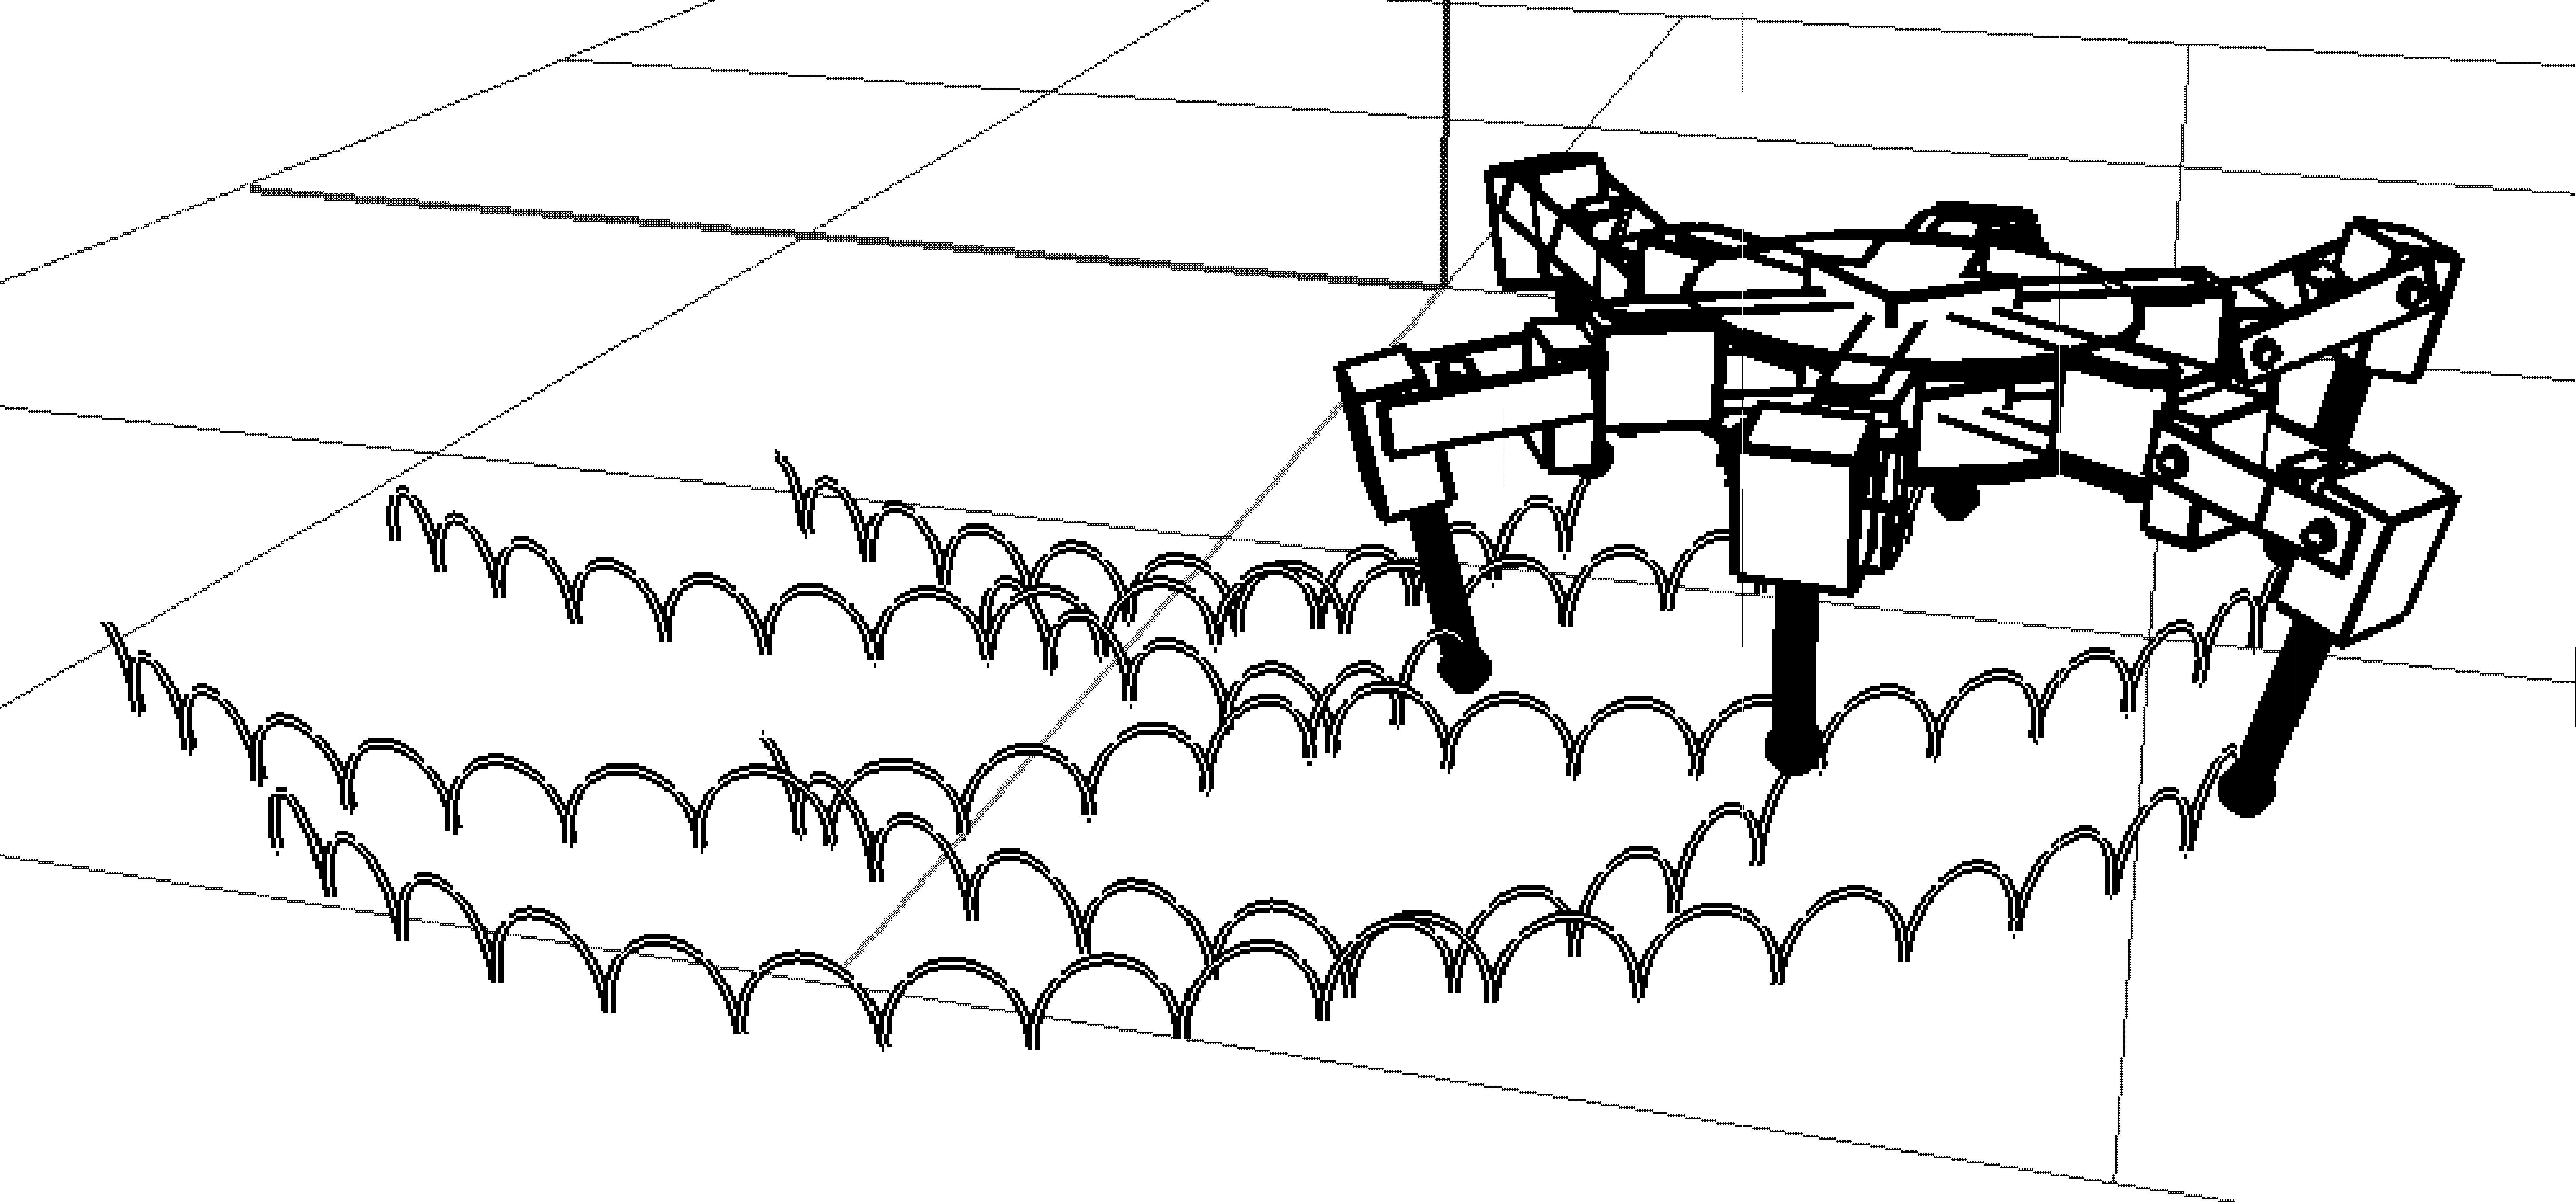
\includegraphics[width = 120mm]{hexa3animation}}}
\caption{Траектории переноса ног в абсолютной системе координат при поступательном движении}
\label{fig:exper1}
\end{figure}

Движение аппарата по окружности с постоянной скоростью равноcильно тому, что угол $\xi$ меняется с постоянной скоростью $\dot{\xi} = \dfrac{2\pi}{30}$, а модуль скорости переноса $V=const$. За время $t=30$с угол $\xi$ линейно изменится от 0 до $2\pi$, т.е. робот пройдёт по окружности ровно за 30 секунд с постоянной скоростью. Величина переносной скорости $V$ определяет радиус окружности по которой пройдёт робот. Вычислим радиус окружности, по которой пройдёт робот. Очевидно, что при заданной скорости $V=0.04$ м/с за время $t=30$ сек робот пройдёт по окружности длинною $l = V\cdot30 = 1.2$метра. Отсюда следует, что радиус траектории $R = 0.19$ метра.
Визуализация траекторий движения (рис. \ref{fig:exper1}) опорных точек ног показывает, что движение происходит без проскальзывания. При поступательном движении все траектории ног равны между собой с точностью до сдвига.

\begin{figure}[t]
\center{\fbox{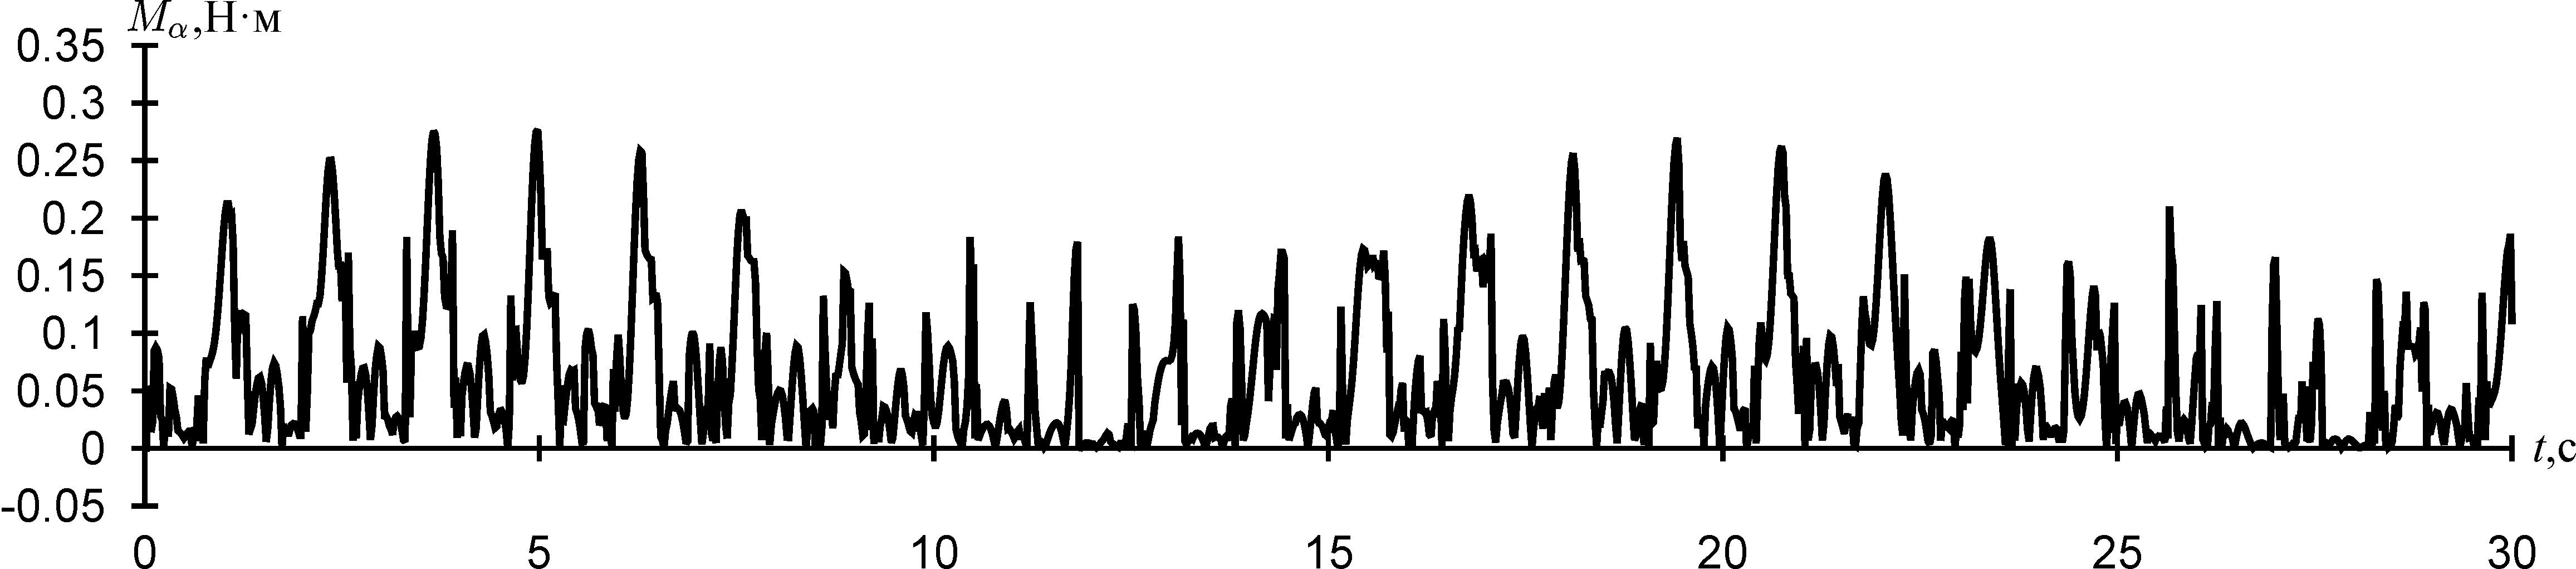
\includegraphics[width=150mm]{hexa3momentalpha}}\\}
\center{\fbox{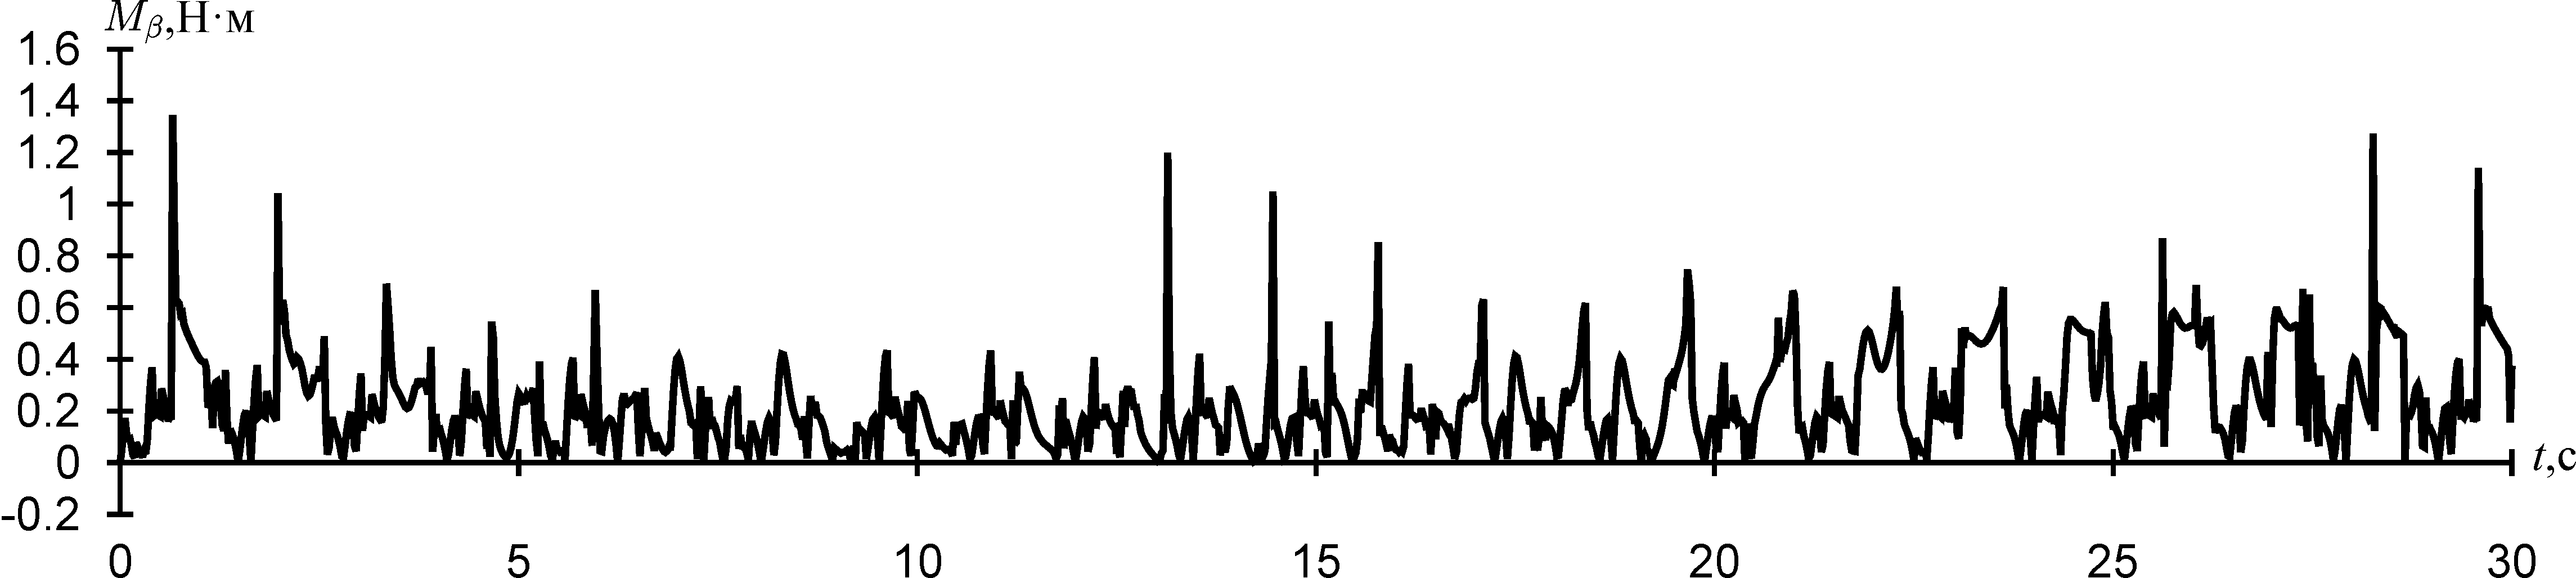
\includegraphics[width=150mm]{hexa3momentbeta}}\\}
\center{\fbox{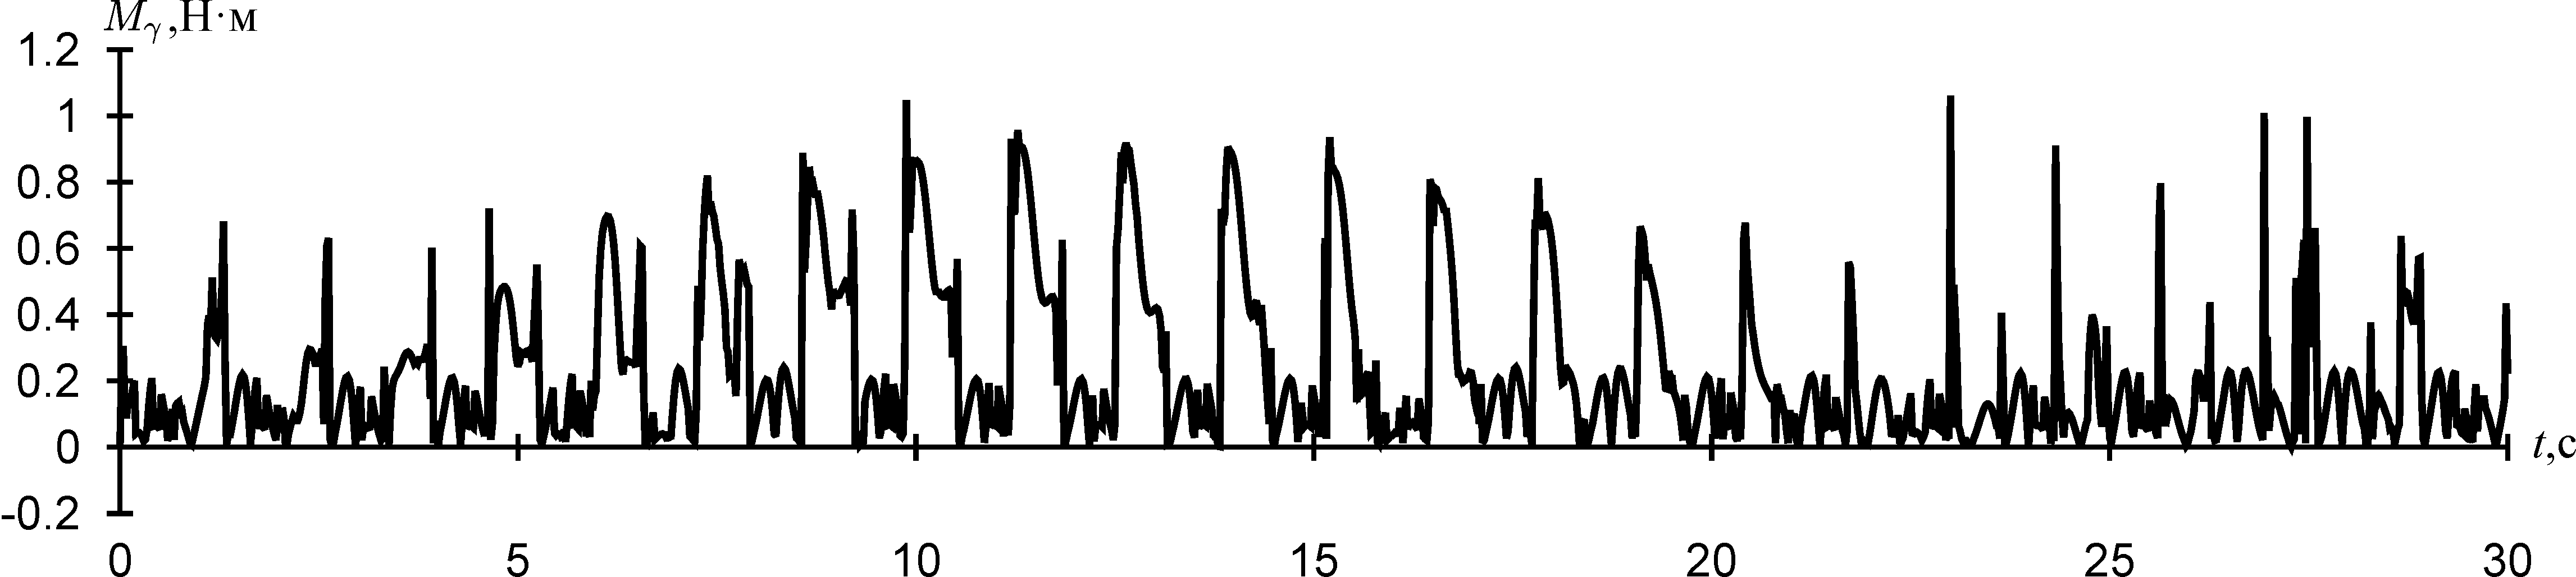
\includegraphics[width=150mm]{hexa3momentgamma}}\\}
\caption{Управляющие шарнирные моменты углов $\alpha, \beta, \gamma$}
\label{fig:exper1moments}
\end{figure}

Из графиков (рис. \ref{fig:exper1moments}) для шарнирных моментов $M_\alpha, M_\beta, M_\gamma$ видно, что наиболее нагруженным является шарнир, соответствующий углу $\gamma$ коленного сустава ноги. Управляющий момент для угла $\gamma$ достигает величины порядка 10~кг$\cdot$см. Самым ненагруженным является шарнир, соответствующий углу $\alpha$. Из графика (рис. \ref{fig:exper1moments}) видно, что шарнирный момент $M_\alpha$ не превышает значение в 3~кг$\cdot$см. Шарнир $\alpha$ отвечает только за перенос аппарата в горизонтальном направлении, на него не происходит распределение веса аппарата.
Возможно, найдётся некоторая оптимальная пара чисел $(x_c, d)$ такая, что сумма $|max M_{\alpha}|+|max M_{\beta}|+|max M_{\gamma}|$ будет минимальна.

\newpage
\begin{figure}[t]
\center{\fbox{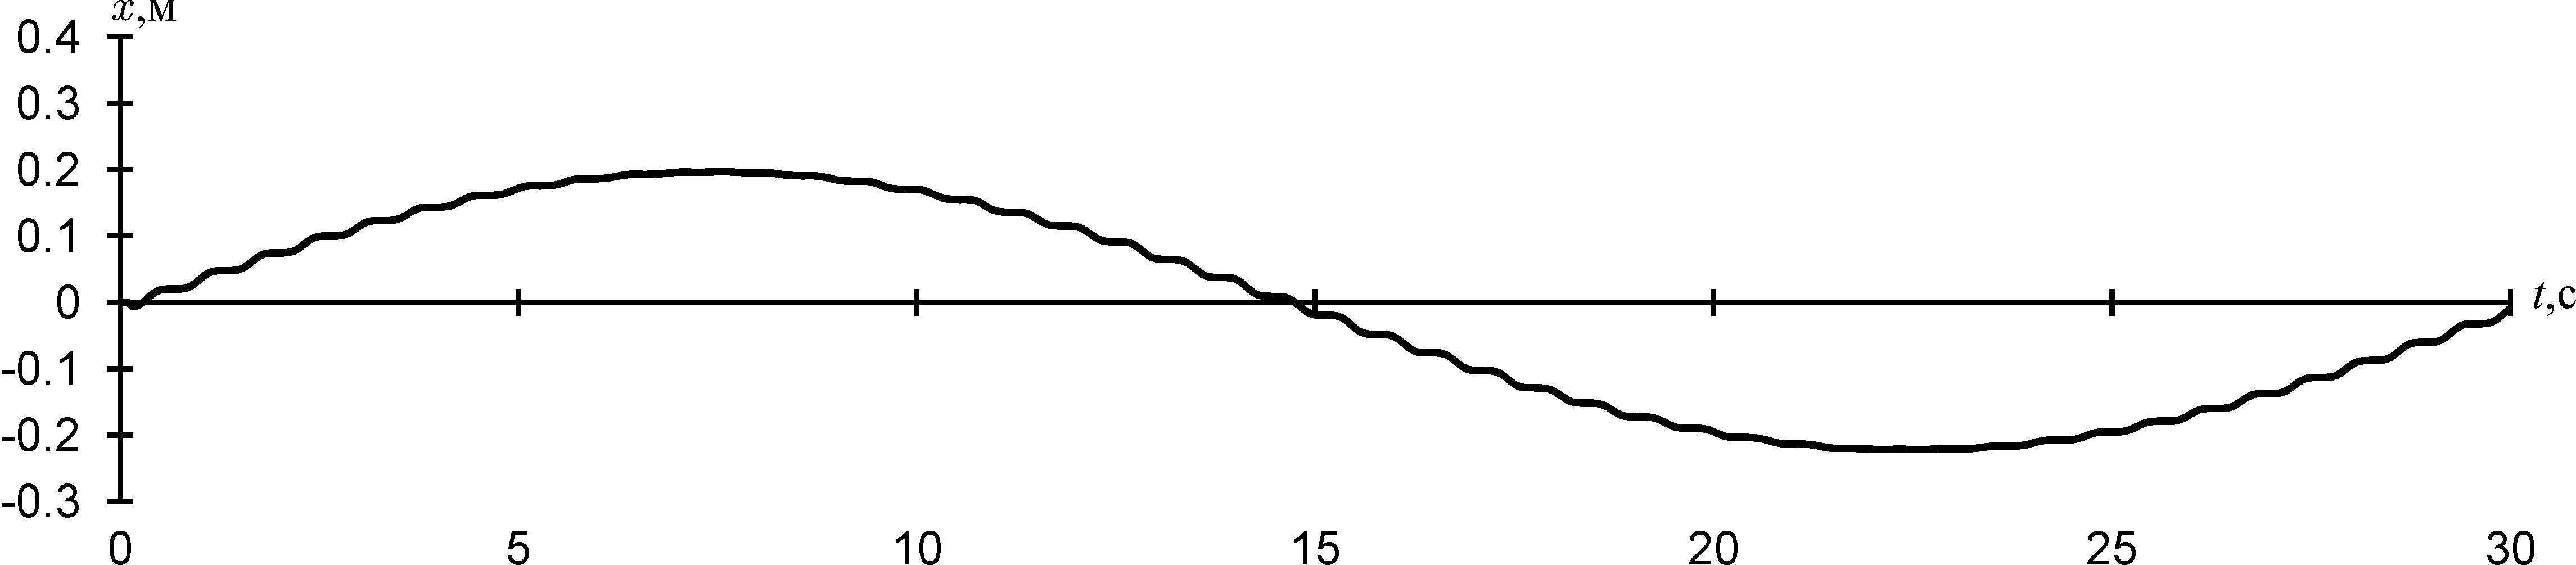
\includegraphics[width=150mm]{hexa3coordx}}\\}
\center{\fbox{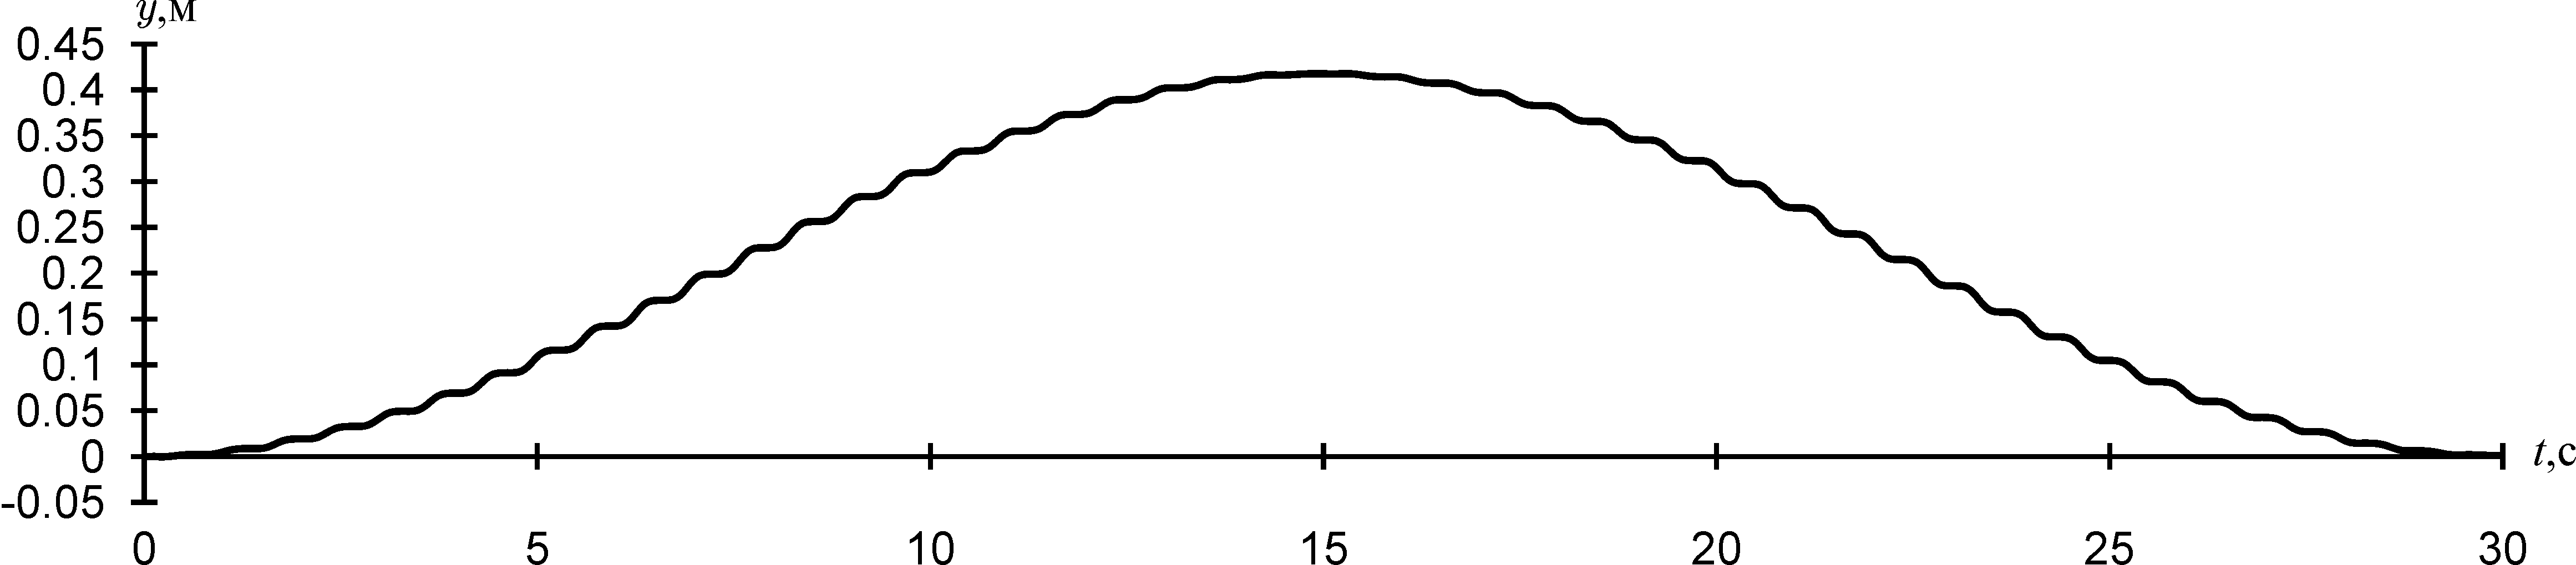
\includegraphics[width=150mm]{hexa3coordy}}\\}
\center{\fbox{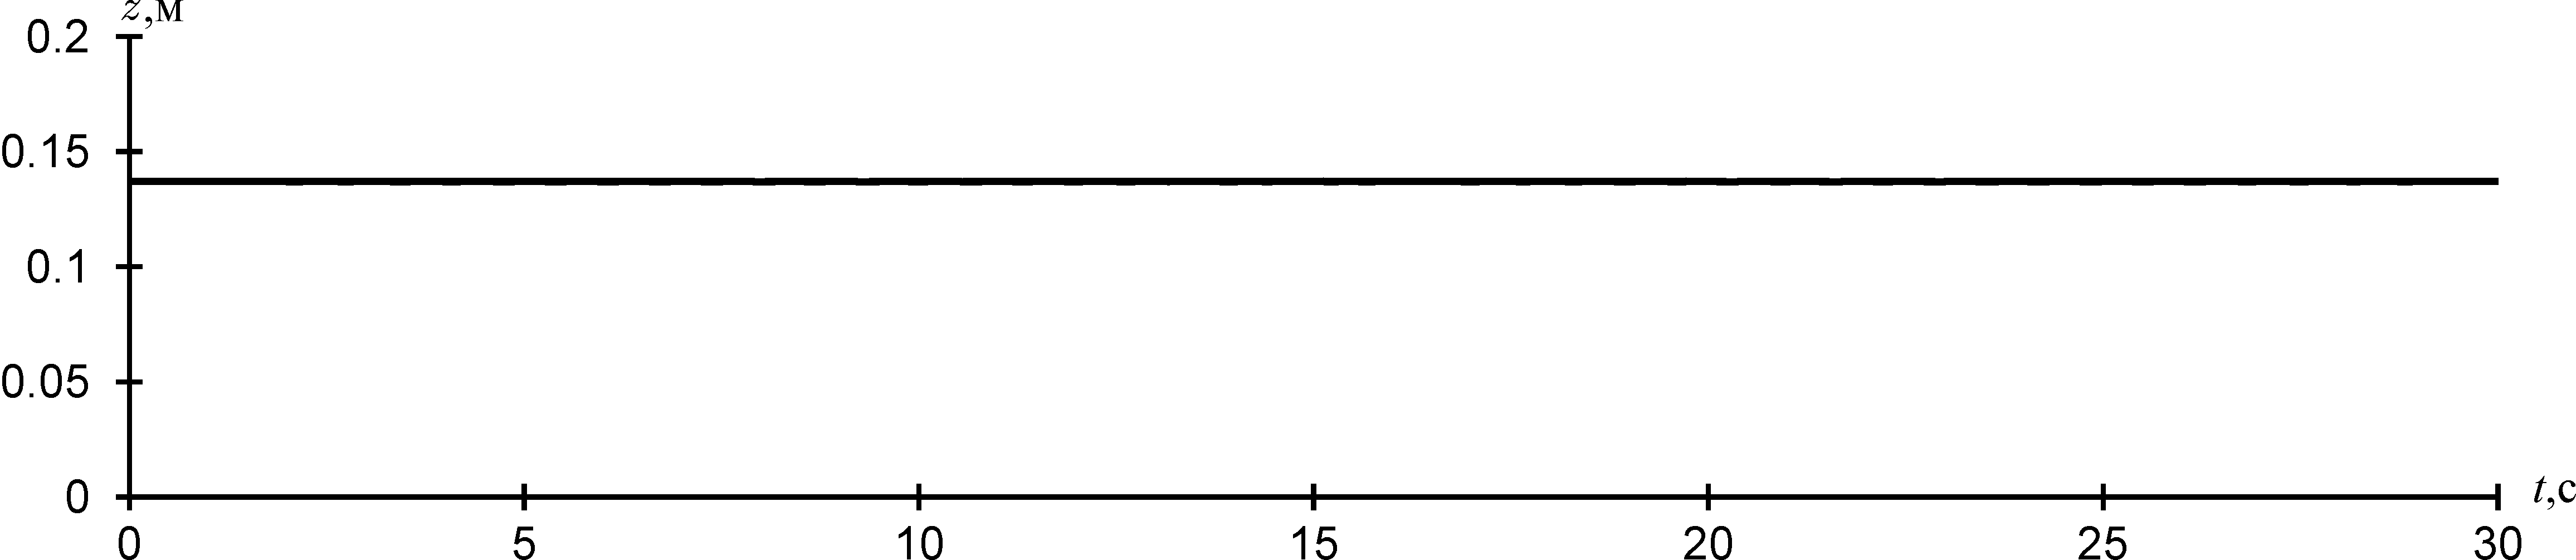
\includegraphics[width=150mm]{hexa3coordz}}\\}
\caption{Координаты центра корпуса $(x,y,z)$}
\label{fig:exper1coord}
\end{figure}

Из графиков (рис. \ref{fig:exper1coord}) видно, что графики $x, y$ имеют ступенчатый вид. Горизонтальные площадки соответствуют моментам времени, когда происходит постановка и съем ног с опорной поверхности. Это прямое следствие выбора параметризации и траектории шагового цикла. Движение робота представляет собой последовательный переход из одной конфигурации ног в другую с обязательной плавной остановкой в моменты смены ног. Фактическая скорость перемещения аппарата постоянно меняется, но средняя величина скорости остаётся постоянной. Из графика для координаты $z$ видно, что корпус робота остаётся на постоянной высоте.

\newpage
\begin{figure}[t]
\center{\fbox{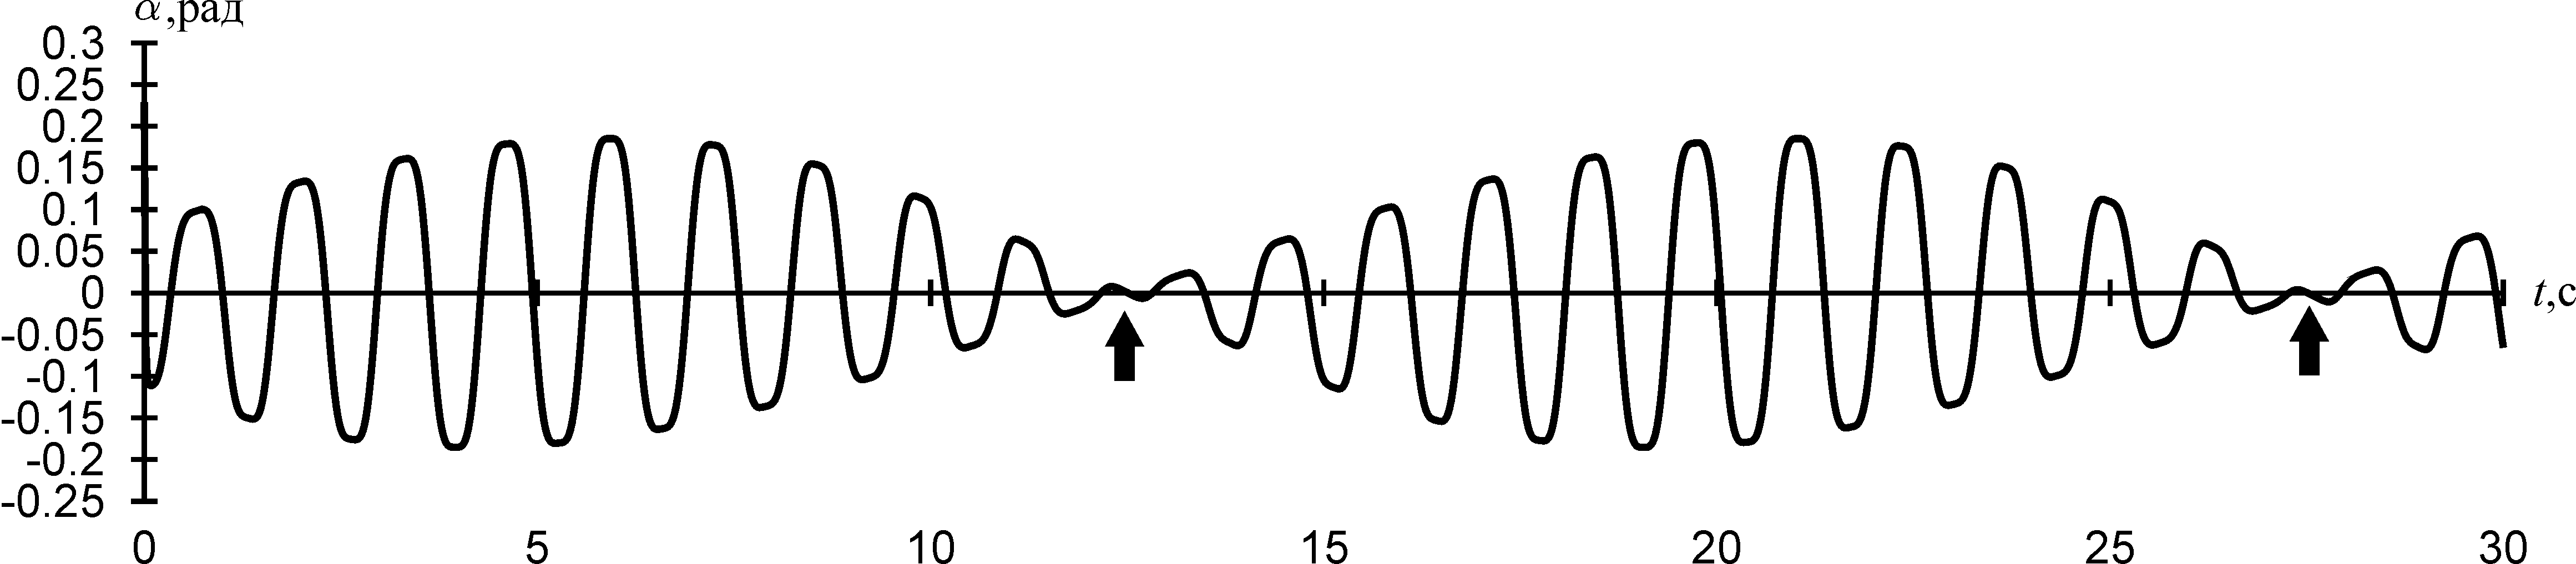
\includegraphics[width=150mm]{hexa3coordalpha}}\\}
\center{\fbox{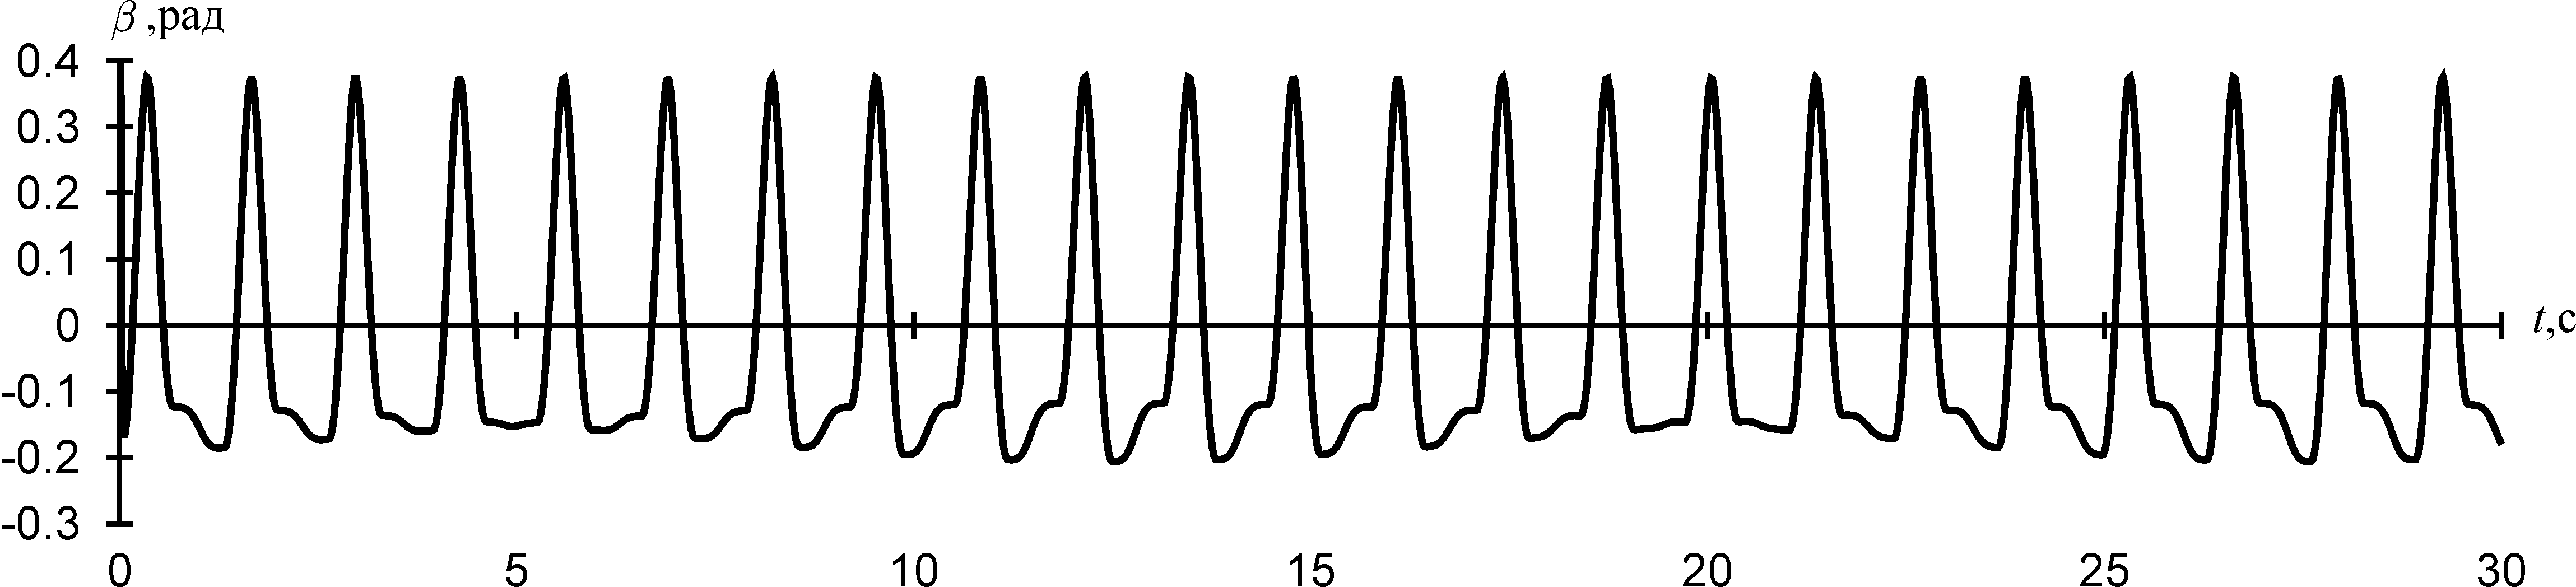
\includegraphics[width=150mm]{hexa3coordbeta}}\\}
\center{\fbox{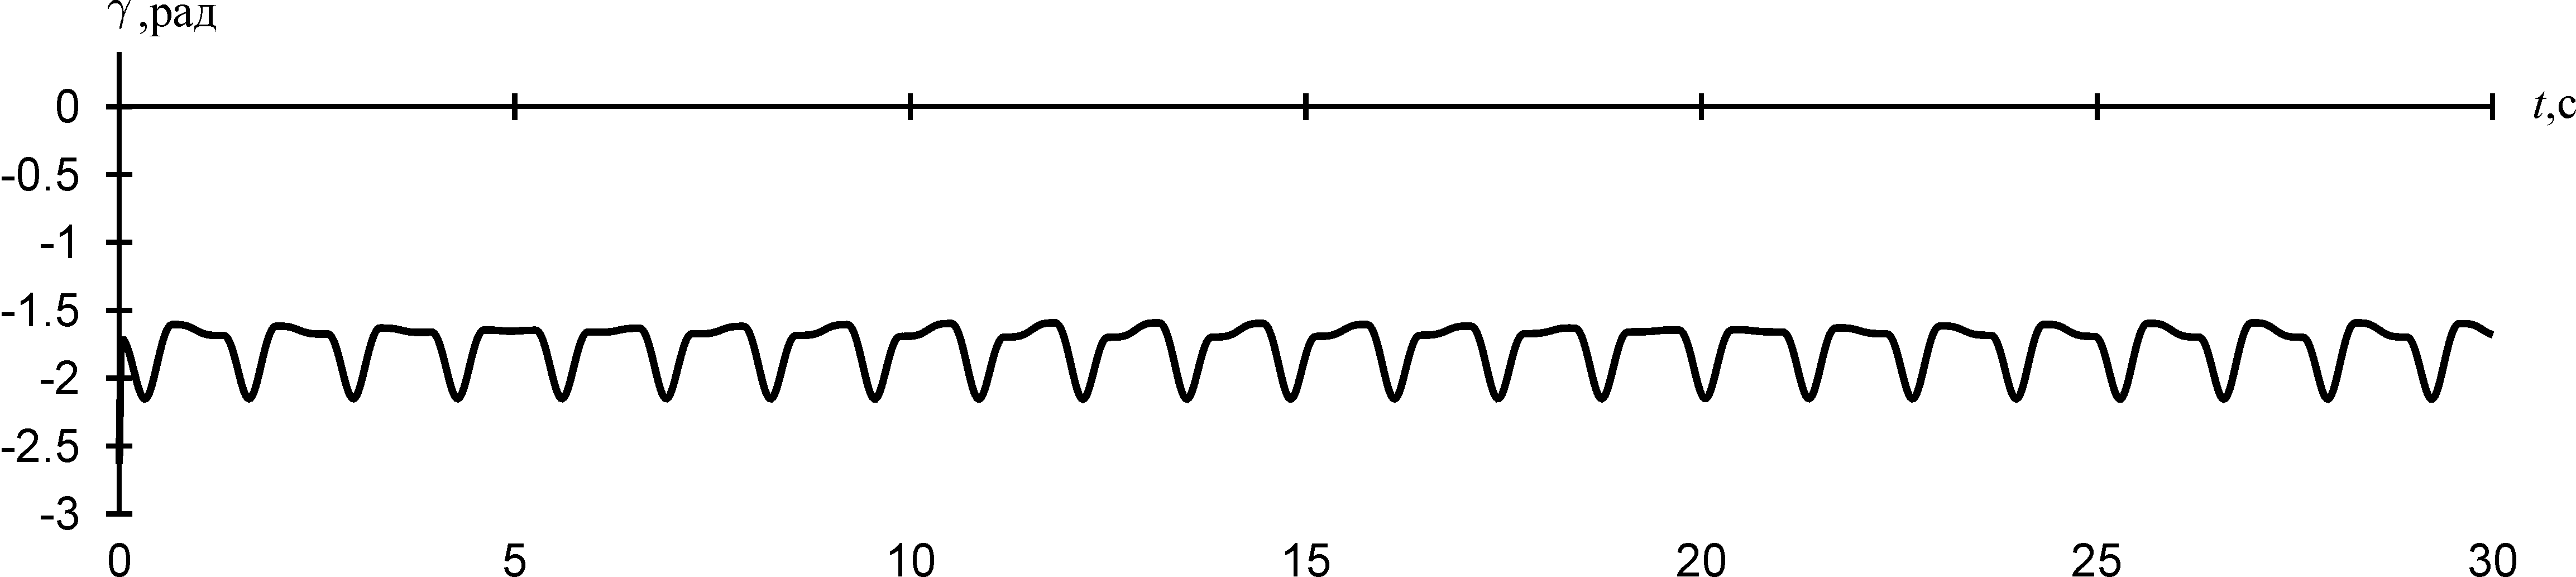
\includegraphics[width=150mm]{hexa3coordgamma}}\\}
\caption{Шарнирные углы $\alpha, \beta, \gamma$}
\label{fig:exper1coord2}
\end{figure}

На графиках для $\alpha, \beta, \gamma$ (рис. \ref{fig:exper1coord2}) явно видна периодичность изменения этих углов. Угол $\alpha$ в моменты времени $t=12,5$с и $t=27,5$с (отмечены на графике стрелками) имеет нулевую амплитуду. Это объясняется тем, что плоскость соответствующей ноги и плоскость, в которой располагается соответствующий шаговый цикл, совпадают. Ноге, чтобы пройти по шаговому циклу, достаточно перемещаться только в своей плоскости. Наибольший диапазон изменения у угла $\beta$, наименьший --- у $\gamma$. Эти диапазоны зависят от макро параметров походки, таких как ширина колеи и высота на которой находится корпус. 

\newpage
\begin{figure}[t]
\center{\fbox{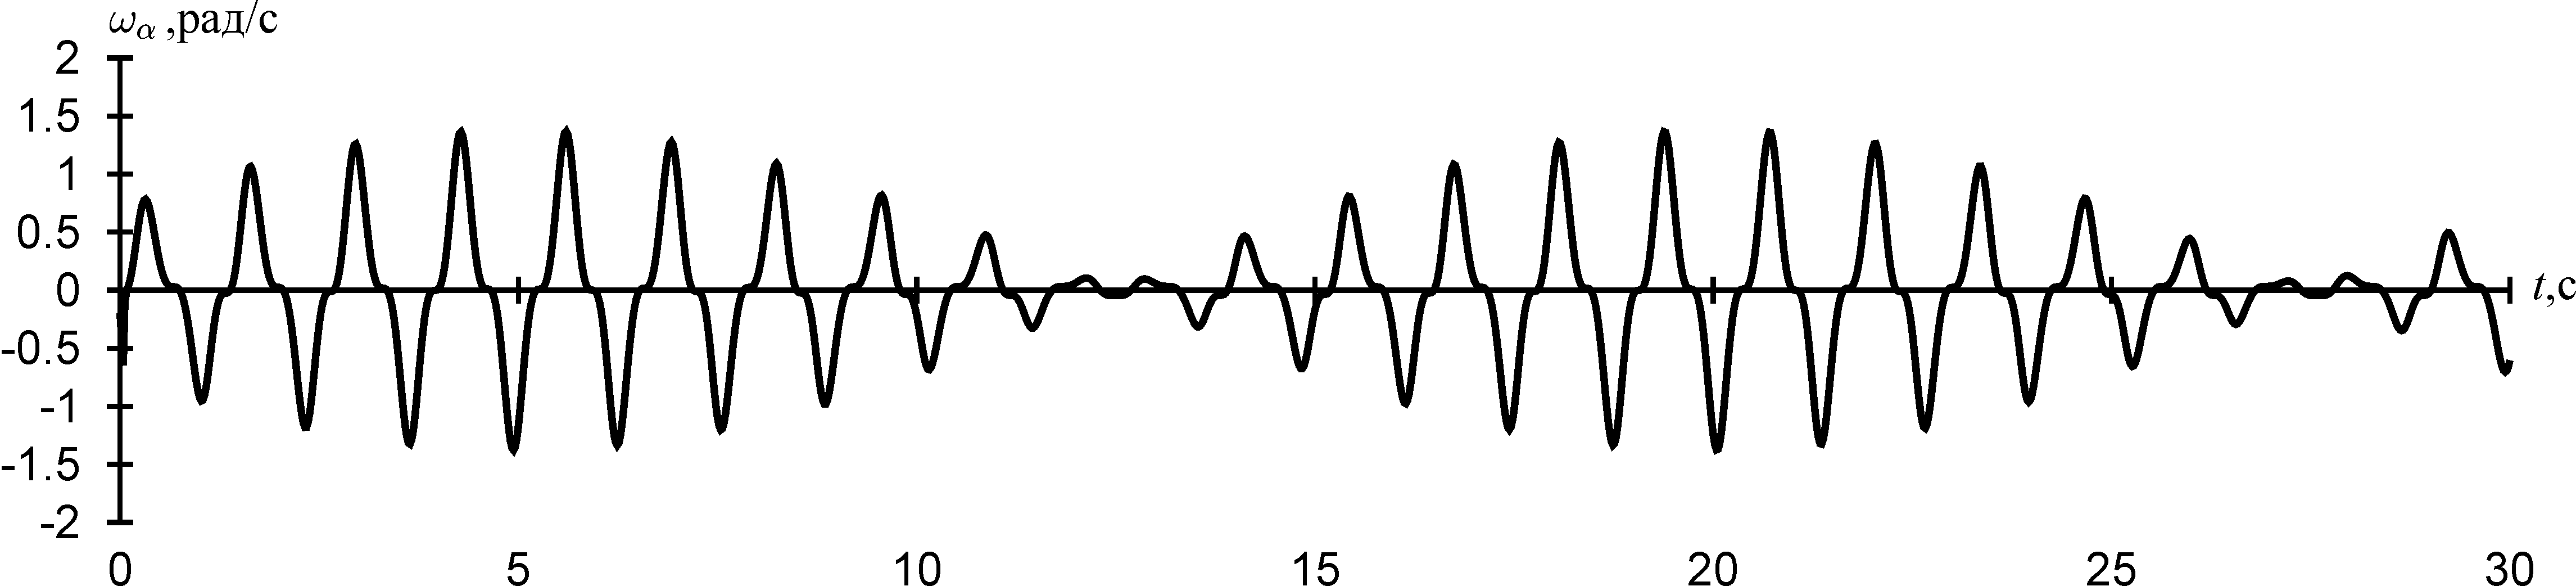
\includegraphics[width=150mm]{hexa3omegaalpha}}\\}
\center{\fbox{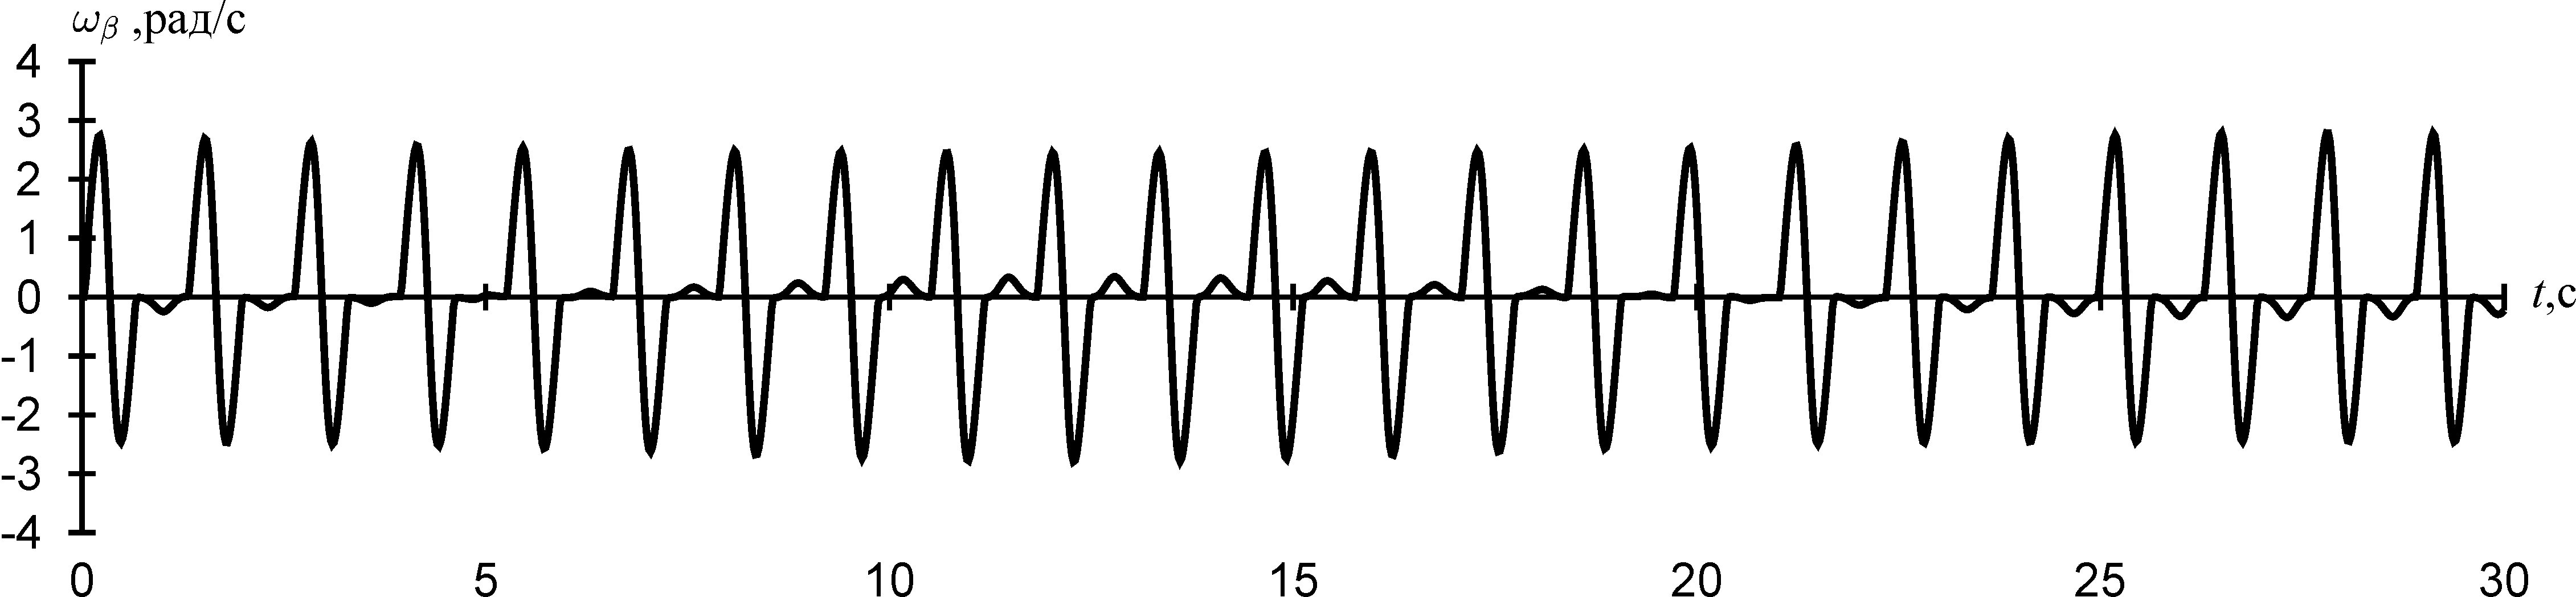
\includegraphics[width=150mm]{hexa3omegabeta}}\\}
\center{\fbox{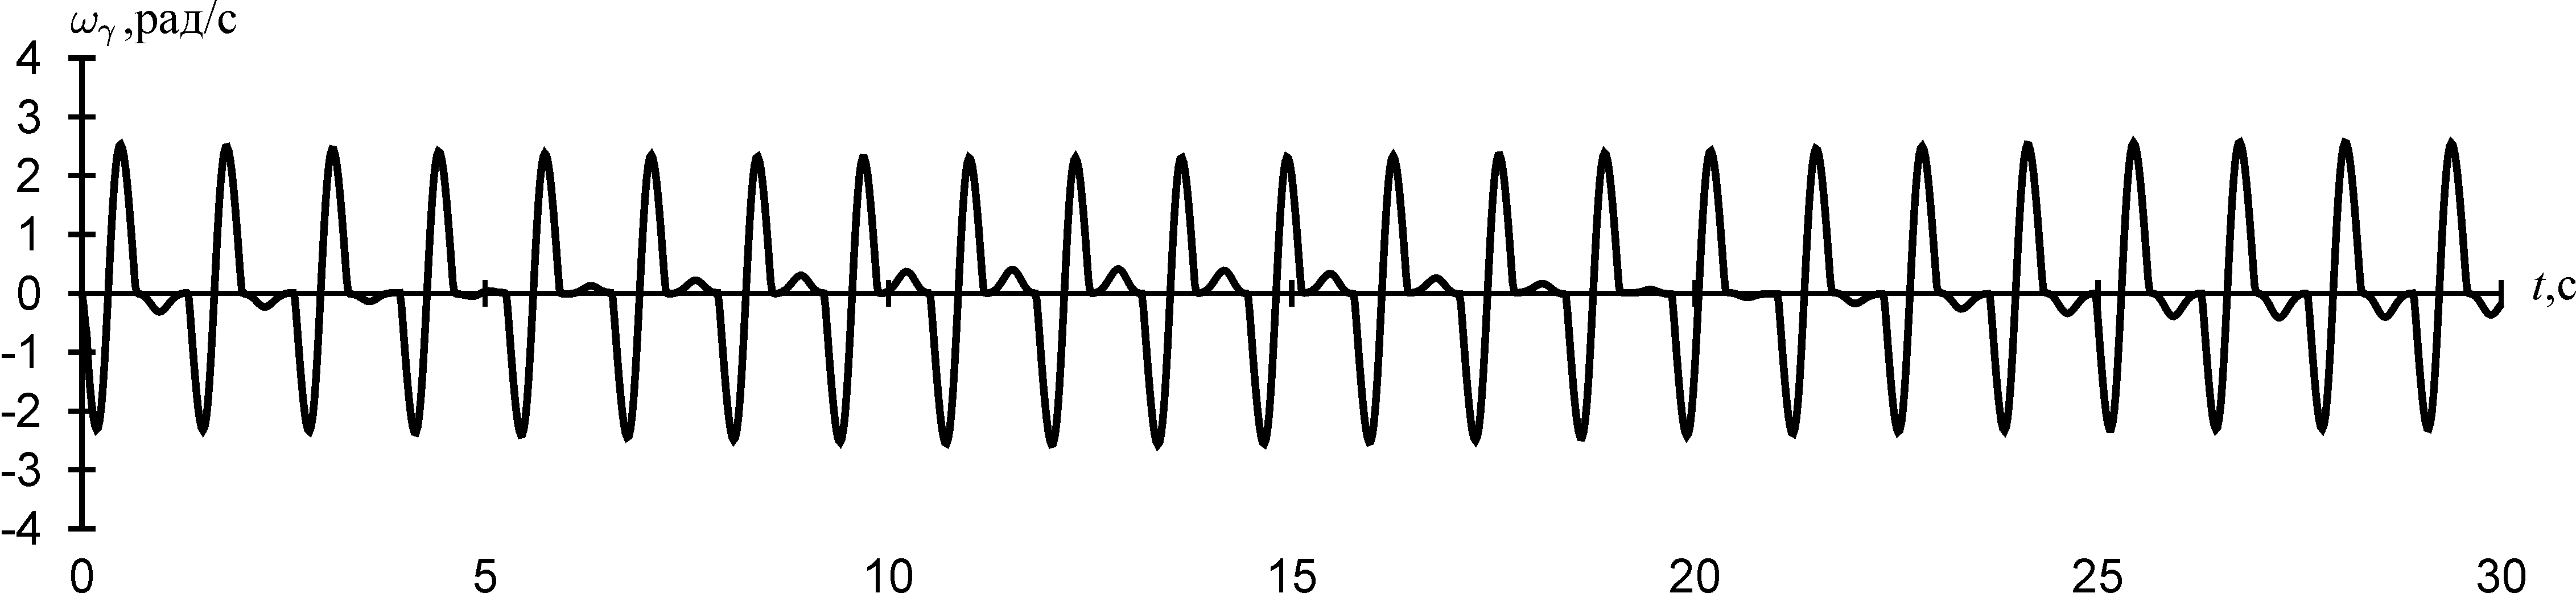
\includegraphics[width=150mm]{hexa3omegagamma}}\\}
\caption{Угловые скорости шарнирных углов}
\end{figure}

Для угла $\alpha$, как следствие из графика (рис. \ref{fig:exper1coord2}), существуют минимумы по амлитуде угловой скорости. Наибольшие угловые скорости возникаются в шарнирах $\beta$ и $\gamma$. Мгновенное значение угловой скорости в этих шарнирах по модулю достигает значения около $170^{\circ}/$с. Ограничения по угловой скорости реальных сервомашинок составляют примерно $90^{\circ}/$с. Это означает, что реальный аппарат не смог бы пройти по аналогичной траектории с аналогичным набором основных параметров шаговых циклов.


\begin{figure}[h]
\center{\fbox{\includegraphics[width=100mm]{blank_pic}\\}
\caption{Кинограмма перемещения аппарата по окружности с сохранением ориентации корпуса}
\end{figure}

\clearpage

\label{sec:exper2}
Движение по окружности с поворотом корпуса задаётся соотношениями:

\begin{center}
$\xi = \omega\,t, \omega = \dfrac{2\pi}{30}, V = 0.057$м/с
\end{center}

\begin{figure}[h]
\newpage
\center{\fbox{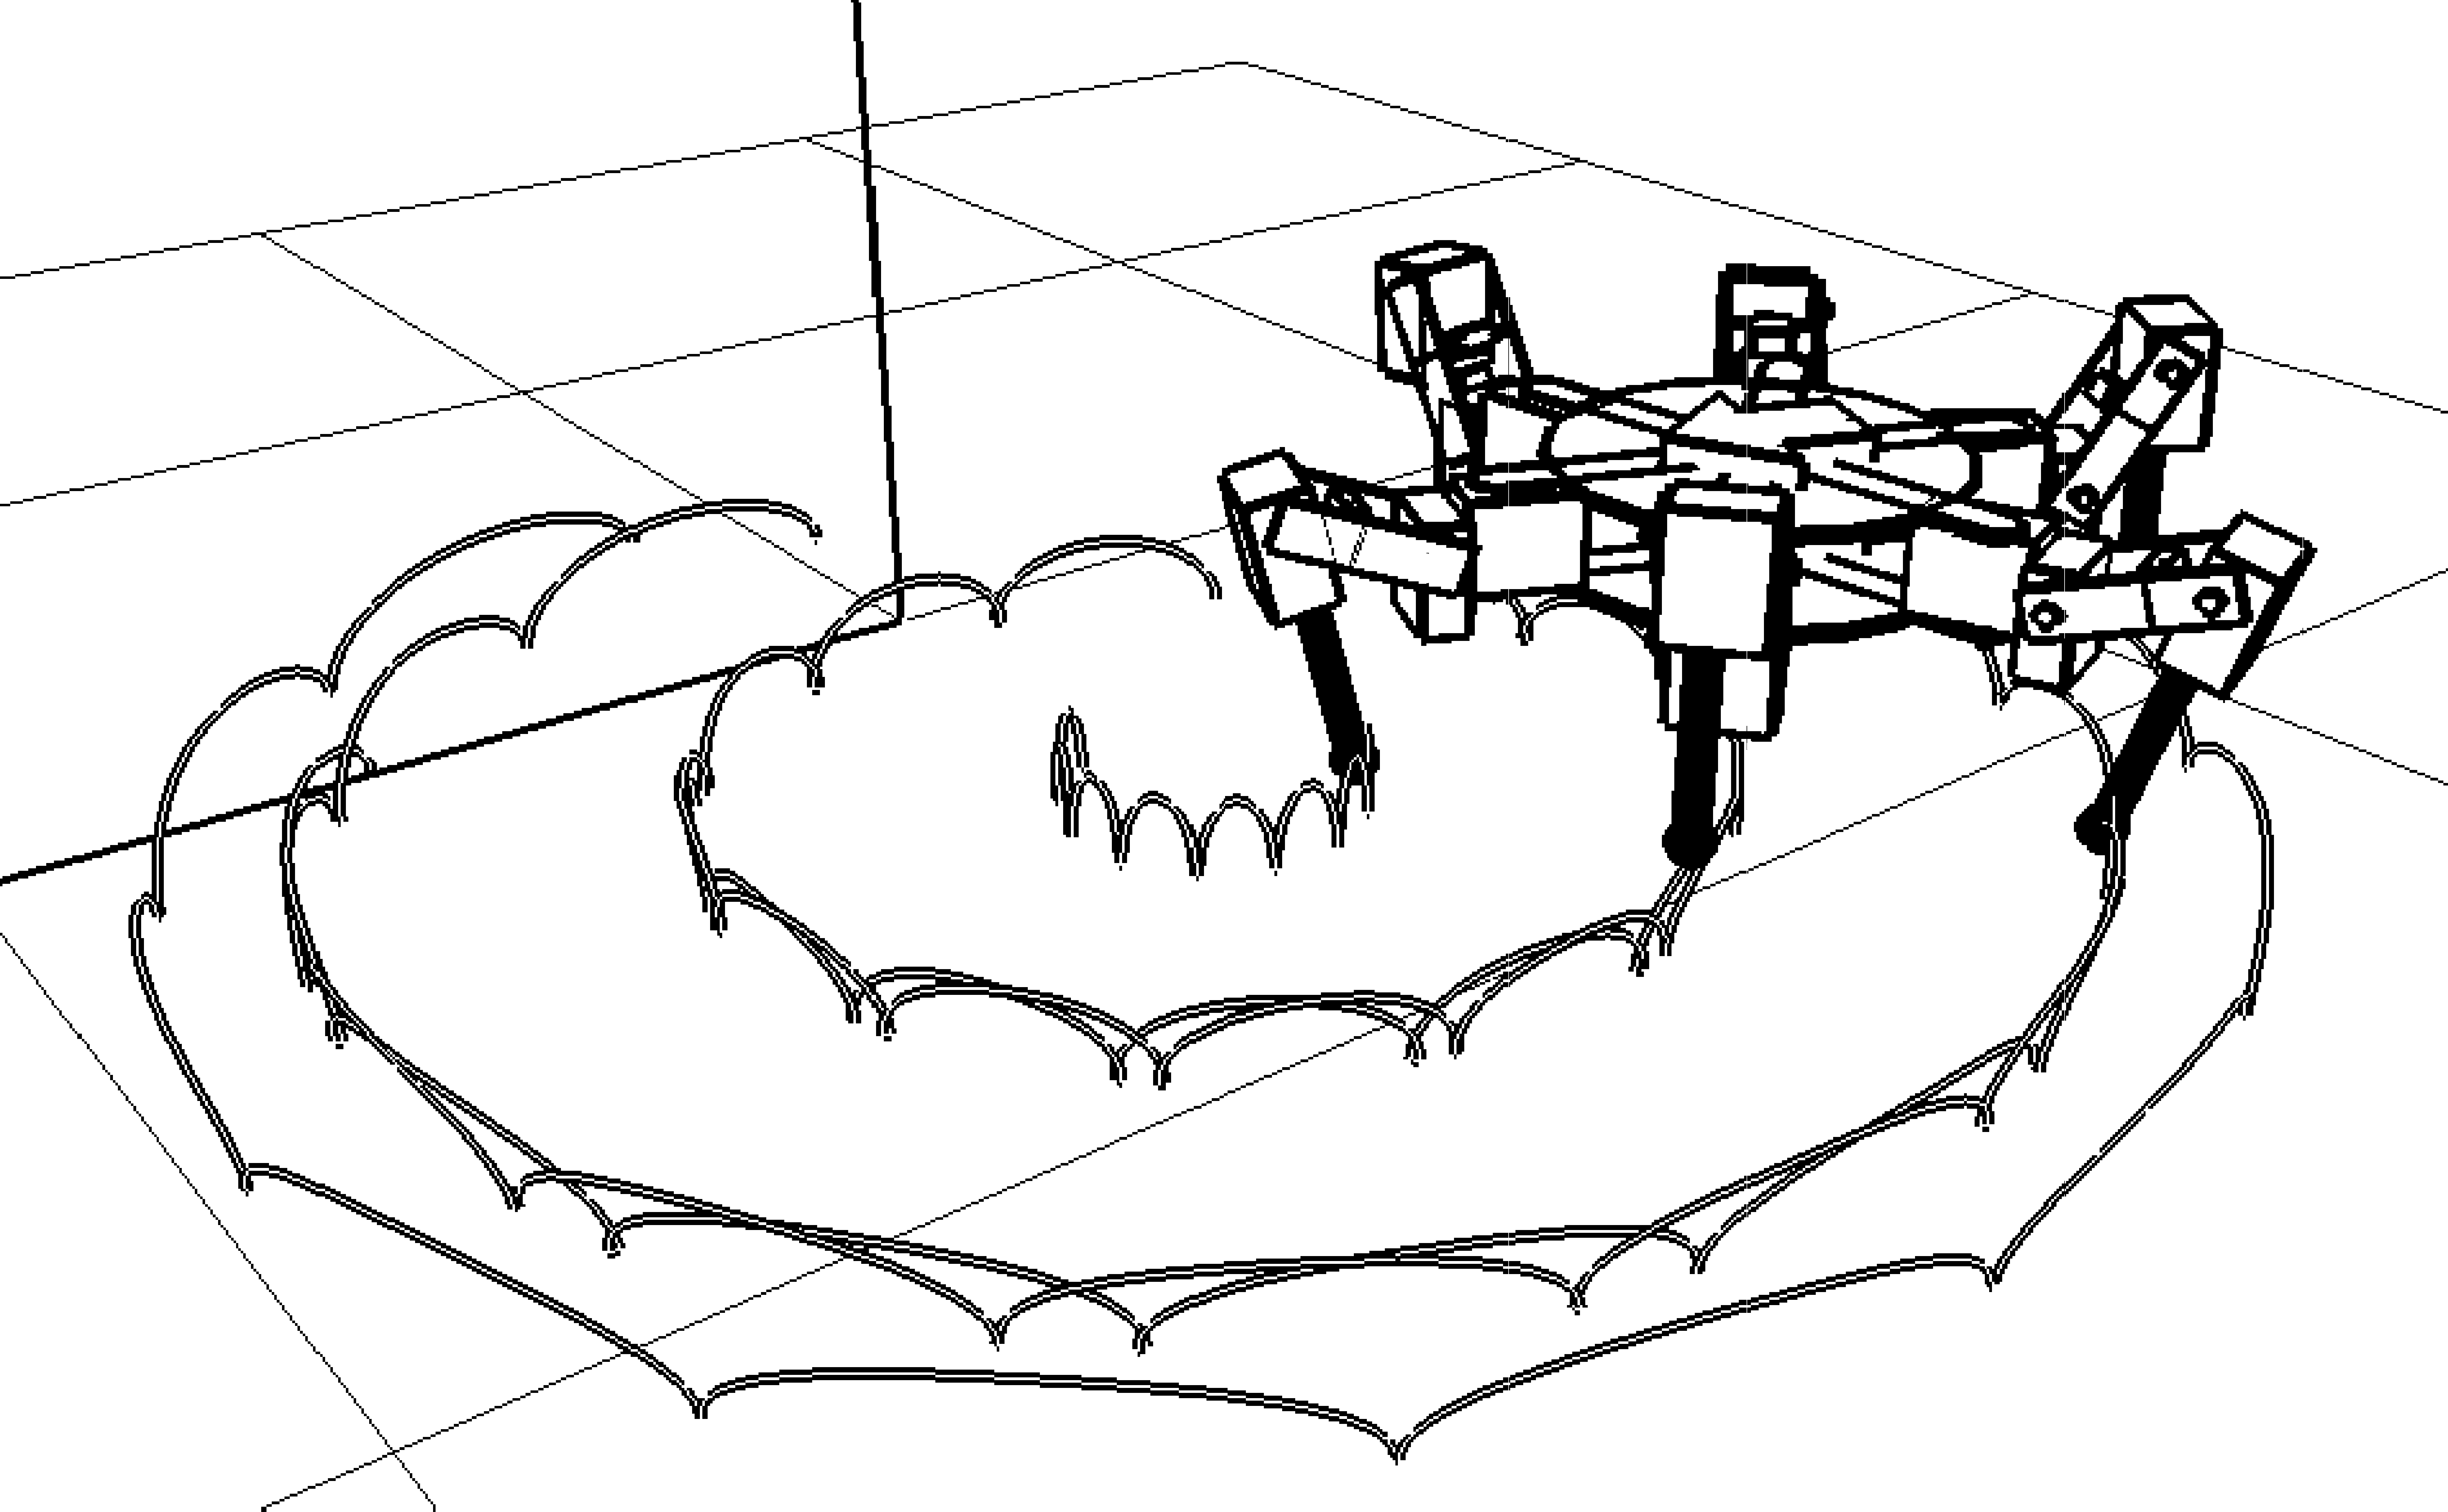
\includegraphics[width=120mm]{hexa4animation}}}
\caption{Траектории переноса ног в абсолютной системе координат при движении с вращением корпуса}
\label{fig:exper2}
\end{figure}

При выбранном соотношении $\dot{\xi}=\omega$ аппарат совершит полный оборот вокруг вертикальной оси одновременно с проходом по окружности. На рисунке \ref{fig:exper2} видно, что шаговые циклы ног различны между собой. Стрелка на верхней крышке корпуса во время движения смотрит всё время в центр заданной окружности. Из построенных траекторий концов ног видно, что движение аппарата происходит без проскальзывания опорных ног.

\newpage
\begin{figure}[t]
\center{\fbox{\includegraphics[width=150mm]{hexa4momentalpha}}\\}
\center{\fbox{\includegraphics[width=150mm]{hexa4momentbeta}}\\}
\center{\fbox{\includegraphics[width=150mm]{hexa4momentgamma}}\\}
\caption{Управляющие шарнирные моменты углов}
\label{fig:exper2moments}
\end{figure}

Шарнирные моменты построены для ноги, совершающей наиболее короткий шаг, на рис.\ref{fig:exper2} это нога, на которую указывает стрелка на верхней крышке аппарата. Указанная нога совершает самый короткий шаг по сравнению с остальными, т.к. находится ближе всего к центру скоростей опорной плоскости. Наибольший шаг совершает нога, наиболее удаленная от центра скоростей. На рисунке \ref{fig:exper2} это нога противоположна ноге, совершающей наименьший шаг.  Как и в параграфе \ref{sec:exper1}, наиболее нагруженным является шарнир, соответствующий углу $\gamma$. На графике момента для угла $\alpha$, в случае движения с вращением корпуса, уже не наблюдается периодических изменений максимальной амплитуды, при каждом шаге нагрузка на шарнир в среднем одинакова.

\newpage
\begin{figure}[t]
\center{\fbox{\includegraphics[width=150mm]{hexa4coordx}}\\}
\center{\fbox{\includegraphics[width=150mm]{hexa4coordy}}\\}
\center{\fbox{\includegraphics[width=150mm]{hexa4coordz}}\\}
\caption{Координаты центра корпуса}
\label{fig:exper2coord}
\end{figure}

На графиках \ref{fig:exper2coord} полная аналогия с графиками на (рис.\ref{fig:exper1coord}), разница только в направлении движения по оси $Oy$ и в радиусе заданной окружности. Графики $x$ и $y$ носят ступенчатый характер, значение координаты $z$ постоянно.

\begin{figure}[h]
\center{\fbox{\includegraphics[width=150mm]{hexa4bodyorientation}}\\}
\caption{Угол ориентации корпуса}
\label{fig:exper2orient}
\end{figure}

На графике (рис. \ref{fig:exper2orient}) построен график угла ориентации корпуса. Отчётливо виден ступенчатый характер графика. Скорость изменения ориентации не постоянна.  

\newpage
\begin{figure}[t]
\center{\fbox{\includegraphics[width=150mm]{hexa4anglealpha}}\\}
\center{\fbox{\includegraphics[width=150mm]{hexa4anglebeta}}\\}
\center{\fbox{\includegraphics[width=150mm]{hexa4anglegamma}}\\}
\caption{Шарнирные углы}
\end{figure}

Шарнирные углы носят индивидуальный рисунок для каждой ноги. Во время движения характер амплитуд колебаний по углам для каждой ноги сохраняется.


\newpage
\begin{figure}[t]
\center{\includegraphics[width=100mm]{kinogramma2}\\}
\caption{Кинограмма движения аппарата по окружности с постоянной угловой скоростью корпуса}
\end{figure}


%\newpage

%\section{Гладкий шаговый цикл}
%\input{hexa_kinematics_new_step_cycle}


%\section{Локальные подвижки корпуса}



%\section{Крен тангаж и рыскание}



\subsection{Заключение}
Моделирование показало эффективность построенного алгоритма управления. Описанный алгоритм управления достаточно прост в теории и не требует больших вычислительных мощностей. Возможно обобщение алгоритма построения опорных траекторий для аппаратов с отличной от инсектоморфной кинематикой ног и с произвольным расположением ног на корпусе.




\chapter{Длинное название главы, в которой мы смотрим на примеры того, как будут верстаться изображения и списки} \label{chapt2}

\section{Одиночное изображение} \label{sect2_1}

\begin{figure} [h] 
  \center
  \includegraphics [scale=0.27] {latex}
  \caption{TeX.} 
  \label{img:latex}  
\end{figure}

%\newpage
%============================================================================================================================
\section{Длинное название параграфа, в котором мы узнаём как сделать две картинки с общим номером и названием} \label{sect2_2}

А это две картинки под общим номером и названием:
\begin{figure}[h]
  \begin{minipage}[h]{0.49\linewidth}
    \center{\includegraphics[width=0.5\linewidth]{knuth1} \\ а)}
  \end{minipage}
  \hfill
  \begin{minipage}[h]{0.49\linewidth}
    \center{\includegraphics[width=0.5\linewidth]{knuth2} \\ б)}
  \end{minipage}
  \caption{Очень длинная подпись к изображению, на котором представлены две фотографии Дональда Кнута}
  \label{img:knuth}  
\end{figure}

%\newpage
%============================================================================================================================
\section{Пример вёрстки списоков} \label{sect2_3}

\noindent Нумерованный список:
\begin{enumerate}
  \item Первый пункт.
  \item Второй пункт.
  \item Третий пункт.
\end{enumerate}

\noindent Маркированный список:
\begin{itemize}
  \item Первый пункт.
  \item Второй пункт.
  \item Третий пункт.
\end{itemize}

\noindent Вложенные списки:
\begin{itemize}
  \item Имеется маркированный список.
  \begin{enumerate}
    \item В нём лежит нумерованный список,
    \item в котором
    \begin{itemize}
      \item лежит ещё один маркированный список.
    \end{itemize}    
  \end{enumerate}
\end{itemize}


\clearpage